\documentclass[usenatbib]{mn2e} 
\usepackage{amsmath} 
\usepackage{amssymb} 
\usepackage{graphics}
\usepackage{graphicx}
\usepackage{epsfig}  
\def\be{\begin{equation}}
\def\ee{\end{equation}}
\def\ba{\begin{eqnarray}}
\def\ea{\end{eqnarray}}

\newcommand{\documentname}{paper~}
\newcommand{\match}{{\tt match}~}
\newcommand{\apj}{ApJ}  
\newcommand{\apjs}{ApJS}  
\newcommand{\apjl}{ApJL}  
\newcommand{\aj}{AJ}  
\newcommand{\mnras}{MNRAS}  
\newcommand{\mnrassub}{MNRAS accepted}  
\newcommand{\aap}{A\&A}  
\newcommand{\aaps}{A\&AS}  
\newcommand{\araa}{ARA\&A}  
\newcommand{\nat}{Nature}  
\newcommand{\physrep}{PhR}
\newcommand{\pasp}{PASP}    
\newcommand{\pasj}{PASJ}    

\newcommand{\kms}{\,km~s$^{-1}$}
\def\squig{\sim\!\!}
\newcommand{\LCDM}{$\Lambda$CDM~}
\newcommand{\beq}{\begin{eqnarray}}  
\newcommand{\eeq}{\end{eqnarray}}  
\newcommand{\zz}{$z\sim 3$} 
\newcommand{\avg}[1]{\langle{#1}\rangle}  
\newcommand{\ly}{{\ifmmode{{\rm Ly}\alpha}\else{Ly$\alpha$}\fi}}
\newcommand{\hMpc}{{\ifmmode{h^{-1}{\rm Mpc}}\else{$h^{-1}$Mpc }\fi}}  
\newcommand{\hGpc}{{\ifmmode{h^{-1}{\rm Gpc}}\else{$h^{-1}$Gpc }\fi}}  
\newcommand{\hmpc}{{\ifmmode{h^{-1}{\rm Mpc}}\else{$h^{-1}$Mpc }\fi}}  
\newcommand{\hkpc}{{\ifmmode{h^{-1}{\rm kpc}}\else{$h^{-1}$kpc }\fi}}  
\newcommand{\hMsun}{{\ifmmode{h^{-1}{\rm {M_{\odot}}}}\else{$h^{-1}{\rm{M_{\odot}}}$}\fi}}  
\newcommand{\hmsun}{{\ifmmode{h^{-1}{\rm {M_{\odot}}}}\else{$h^{-1}{\rm{M_{\odot}}}$}\fi}}  
\newcommand{\Msun}{{\ifmmode{{\rm {M_{\odot}}}}\else{${\rm{M_{\odot}}}$}\fi}}  
\newcommand{\msun}{{\ifmmode{{\rm {M_{\odot}}}}\else{${\rm{M_{\odot}}}$}\fi}}  
\newcommand{\lya}{{Lyman$\alpha$~}}
\newcommand{\clara}{{\texttt{CLARA}}~}
\newcommand{\rand}{{\ifmmode{{\mathcal{R}}}\else{${\mathcal{R}}$ }\fi}}  
\newcommand{\Lsun}{\mbox{\,$L_{\odot}$}}
\newcommand{\like}{\mathscr{L}}
\newcommand{\bftheta}{\mathbf{\Theta}}
\newcommand{\degree}{\ensuremath{^\circ}}
\def\spose#1{\hbox to 0pt{#1\hss}}
\def\simlt{\mathrel{\spose{\lower 3pt\hbox{$\mathchar"218$}}
     \raise 2.0pt\hbox{$\mathchar"13C$}}}
\def\simgt{\mathrel{\spose{\lower 3pt\hbox{$\mathchar"218$}}
     \raise 2.0pt\hbox{$\mathchar"13E$}}}
\font\smcap=cmcsc10

\begin{document}

\title[Dark Matter Halo Mass for LAEs  at $z=3.1$]{Using cosmic
  variance to constrain the dark matter halo mass of Lyman-alpha
  emitting galaxies at $z$=3.1} 
  
\author[~J.~E. Forero-Romero and J. Mejia]{
\parbox[t]{\textwidth}{\raggedright 
Jaime E. Forero-Romero$^{1}$ and
Julian Mej\'ia$^{2}$ 
}
\vspace*{6pt}\\
$^{1}$ Departamento de F\'{i}sica, Universidad de los Andes, Cra. 1
No. 18A-10, Edificio Ip, Bogot\'a, Colombia \\
$^{2}$ --}

\maketitle

\begin{abstract}
We use cosmological N-body simulations to find the characteristic mass
of dark matter halos hosting Lyman-Alpha Emitting (LAE) galaxies at a
redshift of $z=3.1$. The method is based on matching the statistics
for the number density between mock and observed fields. The mock
catalogs are constructed using a simple model where a dark matter halo
can only host one LAE with a probability $f_{\rm occ}$ if its mass is
found withing a certain range mass range delimited by two threshold
values, $M_{\rm min}$ and $M_{\rm max}$. We find that the most of the models that
are consistent the observed cosmic variance statistics are those with
halo masses in the range $10.5 < \log_{10} M_{\rm  min}/hMsun < 11.5$
and $\log_{10} M_{\rm max}/\hMsun < 13.5$ with and occupation fraction
that scales as $f_{\rm occ}=$. We explore three additional constraints
to narrow down these range: the number of mocks consistent with 
observations, observational constraints on the occupation fraction and
the angular correlation function. The first two conditions narrow down
the space parameter to $M_{\rm min}=$ and $M_{\rm max}$, $f_{\rm occ}$. The angular
correlation function does not add a significant constraint due to the
cosmic variance in the small angular fields where this statistics has
been computed so far. We make available the mock data for the best
models in a public repository. Implications for galaxy formation
models? 
\end{abstract}

\begin{keywords}
{galaxies: kinematics and dynamics, Local Group, methods:numerical}
\end{keywords}


\section{Introduction}

Lyman-$\alpha$ emitting galaxies (LAEs) have become in the last decade a 
central topic in studies of structure formation in the Universe. They 
are helpful in a diverse range of fields. LAEs can
be used as probes of reionization \citep{Dijkstra11}, tracers of
large scale structure \citep{Koehler2007}, 
signposts for low metallicity stellar populations and markers of the
the galaxy formation process through cosmic history \citep{ForeroRomero2012}.  


At the same time, theoretical and observational developments have
contributed to the emergence of a paradigm to describe structure
formation in a cosmological context. In this context it is considered
that dominant matter content of the Universe is to be found in dark
matter, whereby each galaxy is hosted by larger dark matter structure
known as a halo. 

Most models of galaxy formation find that the mass of the halo can be
used to predict properties of the galaxy such as its stellar mass and
star formation rate \citep{Behroozi2012}. Processes that regulate the
star formation cycle are also though to be strongly dependent on its
mass. Furthermore, the spatial clustering of galaxies on large scales
is entirely dictated by the halo distribution.  For the reasons
mentioned above, finding the typical dark matter halo mass hosting
LAEs represents a significant step forward to understand the nature of
this population in the context of Lambda Cold Dark Matter
($\Lambda$CDM) paradigm.  

Some theoretical approaches to this problem have been based on a
forward modeling. Starting from the DM halo population, the
corresponding intrinsic star formation properties are infered and
statistics such as the luminosity function, the correlation function
and the equivalent width distributions. Such modelling has been
implemented from analytic considerations, semi-analytic models
 and 
full N-body hidrodynamical simulations
\citep{Dayal2009, ForeroRomero2011, Yajima2012, ForeroRomero2012} . 

Added to the uncertainties in the astrophysical processeses describing
star formation in galactic populations, a highly debated steps in this
approach is the calculation of the fraction of Lyman-$\alpha$ photons
that escape the galaxy to the observer. Given the resonance nature of
the line, the radiative transfer of Lyman-$\alpha$ is sensitive to the
density, temperature, topology and kinematics of the neutral Hydrogen
in the interstellar medium (ISM) \citep{Neufeld1991, ForeroRomero2011,
Laursen2013}.  

This complexity makes the use of monte-carlo simulations for the
radiative transfer a required tool to obtain physically sound results,
although the degeneracy in the physical parameters involved in the
problem makes it difficult to achieve a robust consensus on what is
the theoretical expected value for the Lyman-$alpha$ escape fraction
in high redshift. 


Throughout this \documentname we assume a $\Lambda$CDM cosmology with the
following values for the cosmological parameters, $\Omega_{m}=0.27$,
$\Omega_{\Lambda}=0.73$ and $h=0.70$, corresponding to the matter
density, vacuum density and the Hubble constant in units of 100 km
s$^{-1}$ Mpc$^{-1}$. 

\section{Methodology}

Our method to constrain the typical mass of a dark matter halos
hosting LAEs at $z=3.1$ is based on the comparison of observational
results on the surface number density and the predictions of a simple
model that uses the outputs from cosmological N-body simulations. 

In the next subsections we describe in detail the four key elements of
this workflow. First, we present the observations we take as a
benchmark. Second, the N-body simulation and the halo catalogs we
use. Third, the simplified model that allows us to translated halo
catalogs into mock LAE observations. Fourth, the statistics we use to
compare observational results against our theoretical predictions.

%In this \documentname we constrain the typical mass of dark matter halos
%hosting LAES at $z=3.1$. Our model is based on the number density
%information obtained in the recent large scale survey presented by XXX
%where XXX LAEs are detected over 7 fields of $\sim 46 \times
%35$Mpc$^{2}h^{-2}$ in area comoving in area corresponding to observed
%fields of $XXX$ deg$^{2}$.  

%Both the spatial distribution and luminosities of the galaxies have,
%at least in a statistical sense, informatio to constrain theoretical
%model of LAEs. The most detailed theoretical models are also faced to
%diverse physical and astrophysical uncertainties in obtaining
%statistical prediction for the Lyman-alpha line. This uncertainties
%are largest impediment to consruct an ab-iitio model for LAEs.  

%In this \documentname we want to step back and reduce the complexity of our
%model, with the sole objective of reproducing the cosmic variance in
%the number density of LAEs. Afterwards we will interpret the
%implications of this result for physical models for Lyman-alpha
%emitting galaxies. 

%Our model is based on the predictions of a large volume high
%resolution N-body simulation describing the gravitational dynamics of
%dark matter. We do not have an strong bias towards the theoretical
%expectation of what the mass of the dark matter halo hosting the
%galaxy should be.  Instead, we fully explore the parameter space of
%our simplified model. The only cut we impose is that observed LAEs do
%not reside in dark matter halos with masses less than 10$^{10}$\hMsun
%[citation].    


%In the following subsections we describe the most relevant features of
%the observational data, the N-body simulation we use, our model and
%its parameters together with the method to compare its predictions
%against observations. 

\subsection{Observational Constraints}

The observational benchamark we use in this paper is the LAE number
density information at $z=3.1$ obtained by the panoramic narrow-band
survey presented by \cite{Yamada2012} from a survey 
%Our observational reference are the recently published results of a
%panoramic survey of LAES at $z=3.1$ by \cite{Yamada2012}. 
%This survey
conducted with the Subaru 8.2m telescope and the Subaru Prime
Focus Camera, which has a field of view covering $34\times 27$ arcmin,
corresponding to a comoving scale of $46\times35$ Mpc $h^{-1}$ at
$z=3.09$. The narrow band filter is centered at $4977$ \AA with a
$77$\AA width, corresponding to the redshift range $z=3.062-3.125$ and
$41$ Mpc $h^{-1}$ comoving scale for the detection of the
Lyman-$\alpha$ line centered at $z=3.09$. The authors report a total of
$2161$ LAEs with an observed equivalent width larger than $190$\AA
over a total survey area of $2.42$ deg$^{2}$, this corresponds to an
averaga surface number density of $0.20\pm 0.01$ arcmin$^{-2}$.  

The survey covered four independent fields. The first is the SSA22
field of $1.38$ deg$^2$ with $1394$ detected LAEs, this field has been
known to harbor a region with a large density excess of galaxies. The
second observed region is composed by the fields Subaru/{\it
  XMM-Newton} Deep Survey (SXDS)-North, -Center and -South, with a 
total of $0.58$ deg$^2$ and $386$ LAEs. The third and fourth fields
are the Subaru Deep Field (SDF) with $0.22$ deg$^2$ and $196$ LAEs,
and the fild arotund the Great Observatory Optical Deep Survey North
(GOODS-N) with $0.24$ deg$^2$ and $185$ LAEs. 
%In Table 1 we summarize
%the values we use in throughout this paper for the each field, covered
%area, measured surface LAE number density and inferred number volume
%density. 

There is abundant observational work done on LAEs at redshift $z=3.1$
\citep{Kudritzki2000,Matsuda2005,Gawiser2007,Nilsson2007,Ouchi2008}.
However, we decide to focus on the data from \cite{Yamada2012} because
it has the largest covered area with homogeneous intrumentational
conditions (telescope, narrow band filter), data reduction pipeline
and conditions to construct the LAE catalog. This ensures that the
number density variations among fields are due only to
astrophysical reasons and not different observational conditions or
criteria to construct the catalogs.

%For instance, having
%different selection criteria on the equivalent width (EW) can change
%the number of LAEs included in the catalog, yielding number densities
%different by a factor of two   
%different criteria on the equivalent width (EW) cuts to construct the
%LAE samples. Different cuts in the EW can change the number of LAEs to
%be included in the catalog. This cuts have an impact on the fainter
%LAEs which are more abundante than brighter ones. Different
%definitions of the EW cuts can yield number densities different by a
%factor of two [REF, I think Yamada has some numbers]. 

%Other
%surveys by XXX an XXX that cover similar regions, but they use
%different criteria on the equivalent width (EW) cuts to construct the
%LAE samples. Different cuts in the EW can change the number of LAEs to
%be included in the catalog. This cuts have an impact on the fainter
%LAEs which are more abundante than brighter ones. Different
%definitions of the EW cuts can yield number densities different by a
%factor of two [REF, I think Yamada has some numbers]. 
 



\subsection{Simulation and Halo Catalogs}

The Bolshoi simulation \citep{Bolshoi} we use in this paper was
performed in a cubic volume of 250 $h^{-1}$ Mpc on a side. It includes
dark matter distribution is sampled using $2048^{3}$ particles, which
translates into a particle mass of $m_{\rm   p}=1.35\times 10^{8}$
$h^{-1}$ M$_{\odot}$.  The cosmological parameters are consistent with
a WMAP5 and WMAP7 data with a  density $\Omega_{\rm m} = 0.27$,
cosmological  $\Omega_{\Lambda}=0.73$, dimensionless Hubble constant
$h=0.70$, slope of the power spectrum $n=0.95$ and normalization of the
power spectrum$\sigma_{8}=0.82$ \citep{Komatsu2009,Jarosik2011}.  

We use halo catalogs constructed with a Friend-of-Friends (FOF)
algorithm with a linking lenght of 0.17 times the interparticle
distance. 
%We have veryfied that the main results we present in this
%paper also hold if instead we use halo catalogs constructed from a the
%Bound Density Maxima (BDM) algorithm \citep{KlypinBDM} that are
%defined to have an density of 200 times the critical density. 
The minimum halo mass in the models we construct in this \documentname
correspond to groups of $\sim 75$ particles. The catalogs were
obtained from the publicly available Multidark database \footnote{{\tt
    http://www.multidark.org/MultiDark/}} \citep{2011arXiv1109.0003R}.
We focus our work on halos more massive than $1\times 10^{10}$\hMsun
that are resolved with at least $70$ particles.


\subsection{A Model to Populate Halos with LAEs}
\label{subsec:mocks}

In our model a dark matter halo can only host one or zero LAE. 
There are three parameters in the model that decide whether a halo can host a
galaxy or not: the lower and upper bouds for the mass range $M_{\rm min}<
M_{\rm h} < M_{\rm max}$ where LAEs reside and the fraction $f_{\rm
  occ}$ of such halos that effectively host a LAE. We do not assign a
luminosity to each each LAE. We are primaraly interested in
constraining the halo mass range hosting detectable LAEs under the
conditions defined by \cite{Yamada2012}. In what follows will describe by
the letter ${\mathcal M}$ a model defined by an specific choice of the
three scalar parameters $M_{\rm min}$, $M_{\rm  max}$ y $f_{\rm occ}$.  


For each model ${\mathcal M}$ we create a set of mock fields from
disjoint volumes in the simulation. Each volume has the same geometry
probed by Suprime-CAM and the narrow band filter, namely rectangular
cuboids of dimensions $46\times 35\times 41$ $h^{-3}$Mpc$^{3}$ where
the last dinemsion goes in the redshift direction. This corresponds to
a total area of $880$ arcmin$^{2}$ in each mock field. We construct a total
$5\times 7 \times 6=210$ of such volumes from a snapshot in the Bolshoi
simulation. In each mock field a LAE is assigned to the position of a
dark matter halo if the halo mass is in the range allowed by the model
$M_{\rm min}<M_{\rm h}<M_{\rm max}$ and a random variable taken from
an homogeneous distribution $0\leq \xi<1$ is smaller than the occupation
fraction $\xi<f_{\rm occ}$.

Next we construct mock surveys by making groups of $11$ mock fields
out of the $210$ available volumes. In total $15$ mock surveys are
constructed for each model $\mathcal{M}$. 
%mock fields into
%sets of $11$ different ways to
%construct the LAEs. The first way (match method) we
The grouping is done in two different ways. In the first way, called
{\texttt match}, we follow
the clustering of the observed fields. From the $11$ mock fields, $7$
are constructed from contigous fields in the simulation to mimic the
SSA22 region, $3$ are also contiguous between them but not to the first
$7$ fields to mimic the SXDS fields and finally $2$ non-contigous
fields to imitate the SDF and GOODS-North field. Our main goal with
this selection is to test the impact on the final statistics of having
$7$ clustered fields. The second way to group the mock fields is called {\texttt
  random}, whereby all the $11$ fields are selected in such a way as
to avoid that any two volumes are contigous.
%follow the observational setup and constructs $15$ different mock
%surveys, each one composed of $12$ mock fields, out of which $7$
%correspond to contiguous sub-boxes in the simulation to mimick the
%whole SSA22, $3$ are also contiguous between them but not to the first
%$7$ fields to mimick the SXDS fields and finally $2$ non-contiguous
%fields that correspond to the SDF and GOODS-North fields. This will
%produce $15$ different distributions for the number density for a
%given model ${\mathrm M}$. The second (random method) is similar to the first
%one. There aare $15$ different mock surveys with $12$ mock fields
%each, but this time each field corresponds to uncorrelated sub-boxes
%in the simulation. The third (full method) way in only has $1$ mock survey
%containing all the $210$ mock fields, in this setup there is only one
%predicted number density distribution for each model ${\mathrm M}$ 
%We create the mock surveys in two different ways. First we follow 
%The advantage of these three sampling ways is that they allow us to
%explore the effects of both cosmic variance and the correlation
%between fields. Comparing the results of the first and second method
%will help us to quantify the effect of field correlation, while
%compating the first and the third method will serve us to gauge the
%impace of cosmic variance. 


\subsection{Sampling and Selecting Models}

We make a thorough exploration of the parameter space for the models
${\mathcal M}$. $\log_{10} M_{\rm min}$ takes $30$ values from $10.0$ up
to $12.9$ with an even spacing of $0.1$ dex. $\log_{10} M_{\rm max}$
takes values in the same range as $\log_{10}M_{\rm min}$ only with a
displacement of $0.1$ dex in the whole range. The occupation fraction
$f_{\rm occ}$ takes $10$ different values from $0.1$ to $1$ regulary
spaced by $0.1$. In total the number of different models ${\mathcal
  M}$ that are explored is $30 \times 30 \times 10 = 9000$.

For each mock survey generated in a given model ${\mathcal M}$ we
compute the surface density in the $12$ mock fields. We perform a
Kolmogorov-Smirnov (KS) to compare this mock date against the $12$
observational values. From this test we obtain a value $0<P<1$ to
reject the null hypotesis, namely that two data sets come from the
same distribution. In this paper we consider that for values $P>0.05$
the two distributions can be thought as coming from the same
distribution.

In this paper we consider that a model
${\mathcal M}$ that has at least one (1) mock survey (out of 15)
consistent with the observed distribution of LAE number densities has
viable parameters thatdeserve to be considered for further analysis.  

%For each mock survey generated in a given model ${\mathcal M}$ we compute the LAE surface density
%distributions for the three different ways of grouping the mock
%fields, as described in the previous section. For each sub-volume we
%project the positions of the LAE hosting halos along the $z$ direction
%and calculate its surface number density in units of sources per
%arcmin$^{2}$. For each number density distribution we perform a
%Kolmogorov-Smirnov against the $12$ surface density observational
%values. From this test we obtain the value $0<P<1$ to reject the null
%hypothesis, namely that the two data sets come from the same
%distribution. In this paper we use values of $P>0.1$ to consider that
%the simulated and observed number densities come from the same
%distribution. 

%We generate a series of models ${\mathcal M}$ with different input
%parameters$\{M_{\rm min}, M_{\rm max}, f_{\rm occ}\}$ as
%follows. $M_{\rm min}$ and $M_{\rm max}$ are allowed to take 30
%different values evenly spaced by $0.1$ dex, $M_{\rm min}$ ranges from
%$\log_{10}M_{\rm min}=10.0$ up to $\log_{10}M_{\rm min}=12.9$, while
%$M_{\rm max}$ range  from $\log_{10}M_{\rm min}=10.1$ up to
%$\log_{10}M_{\rm min}=13.0$. The occupation fraction $f_{\rm occ}$
%takes 100 different values from $0.01$ to $1.00$ regularly spaced by
%$0.01$. In total the number of different sets of input parameters to
%be explored is $30 \times 30\times 100 = 9\times 10^{4}$. 

\section{Basic Results}


\begin{figure}
\begin{center}
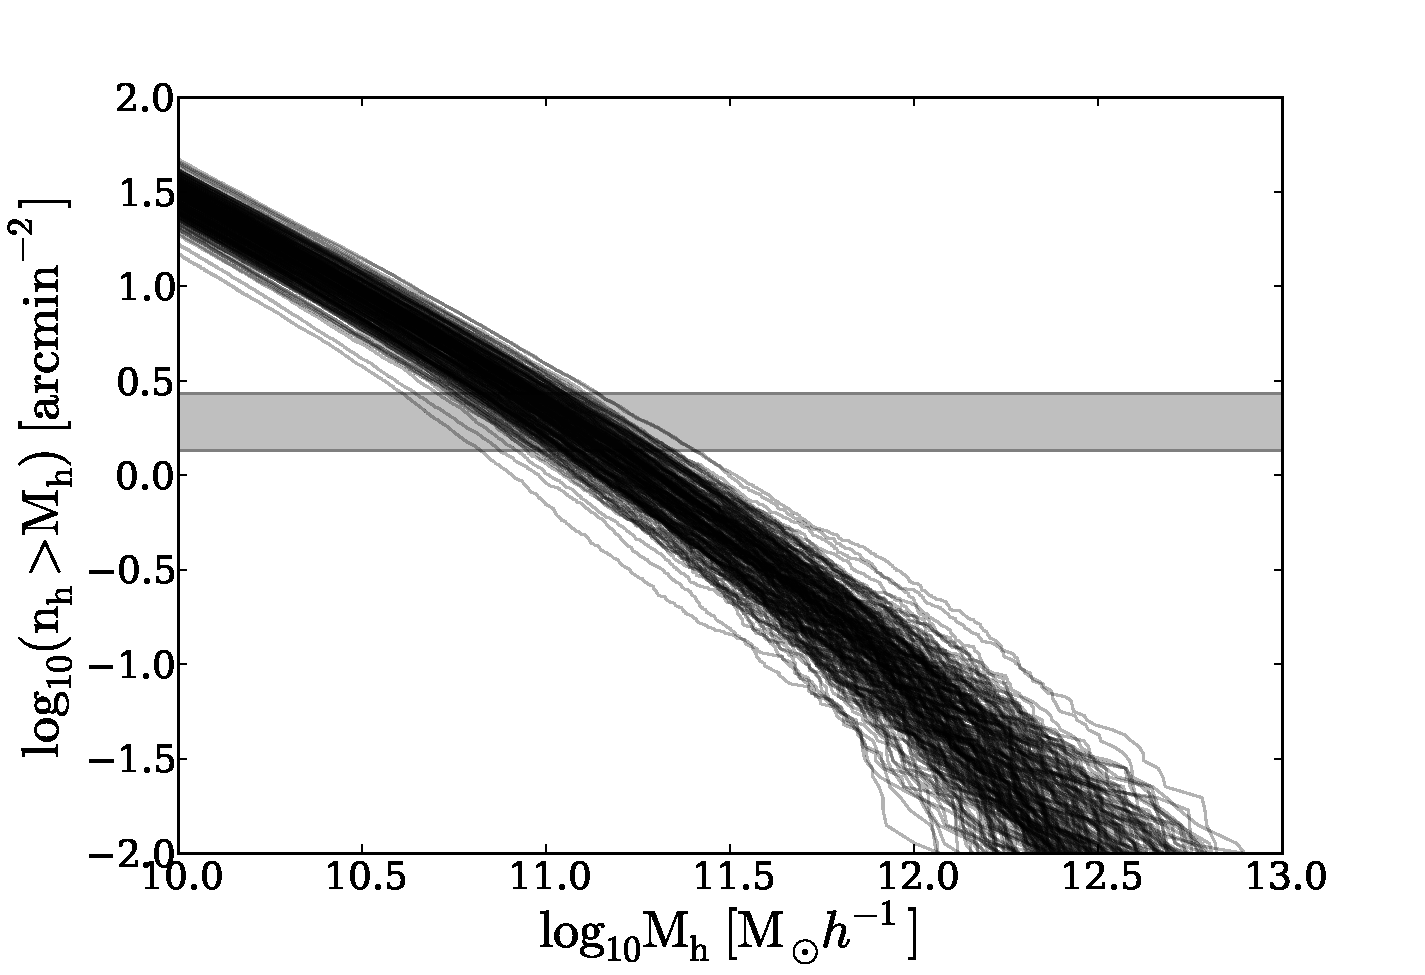
\includegraphics[width=1.10\linewidth,angle=0]{./plots/Fig1.pdf}
\caption{ \label{fig:halos} Surface density of dark
  matter halos as a function of a minimum halo mass to count the
  total number of elements in a volume. Each line represents on of the
  $210$ volumes of dimensions $46\times 35\times 41$ h${-3}$Mpc$^{3}$
  in the Bolshoi simulation. The horizontal grey band represents the
  range of surface densities observed for LAEs at $z=3.1$ as reported
  by \citep{Yamada2012}.}
\end{center} 
\end{figure}


\subsection{Dark Matter Halo Number Density}

In Figure \ref{fig:halos} we present the results for  the
integrated dark matter halo surface density as a function of halo
mass. Each line corresponds to one of the 210 sub-volumes in the
Bolshoi simulation. The gray band indicates the surface density
values for LAEs allowed reported in observations \citep{Yamada2012}.
 
This result provides the basis to understand why a range of models
${\mathcal M}$ can be expected to be consistent with
observations. In Figure \ref{fig:halos} we can read that models
with a minimum mass $\log_{10} M_{\rm min}>11.5$\hMsun will always have a
surface number density lower than the observational
constrain. The oppossite is true in models with $\log_{10} M_{\rm min}<10.5$
that will show surface number density larger than observations, this
implies that in such models the occupation fraction has to be tuned
$f_{\rm occ}<1.0$ as to lower the halo numeber density to match the
gray band values.

%This basic result provides the basis to understand the range of models
%${\mathcal M}$ expected trends for the
%LAEs' preferred mass and the occupation fraction.  
%From this Figure we
%can read which models do not have achance reproduce the
%observations. Regions in the plot where the halo surface density
%values are below the observational constraint correspond to high
%masses halo masses. For a LAE model ${\mathcal M}$ with a minimum mass
%$M_{\rm   min}> 3 \times 10^{11}$\hMsun located inthat mass range, the
%surface density is too low compared with observations.   

Conversely, there are regions in the plot where the halo surface
density is always higher than the observational constraints correspond
to models ${\mathcal M}$ with a minimum mass below $M_{\rm min}<
3\times 10^{10}$\hMsun. Models with this minimum mass hava a chance
for successfuly reproducing observations if the occupation fraction
$f_{\rm occ}<1$ is tuned as to lower the halo number density down to
the observed value.    

In the next subsection we quantify this intuition by means of the KS
tests between mock surveys and observations.

\subsection{Three Regions in Parameter Space}

\begin{figure*}
\begin{center}
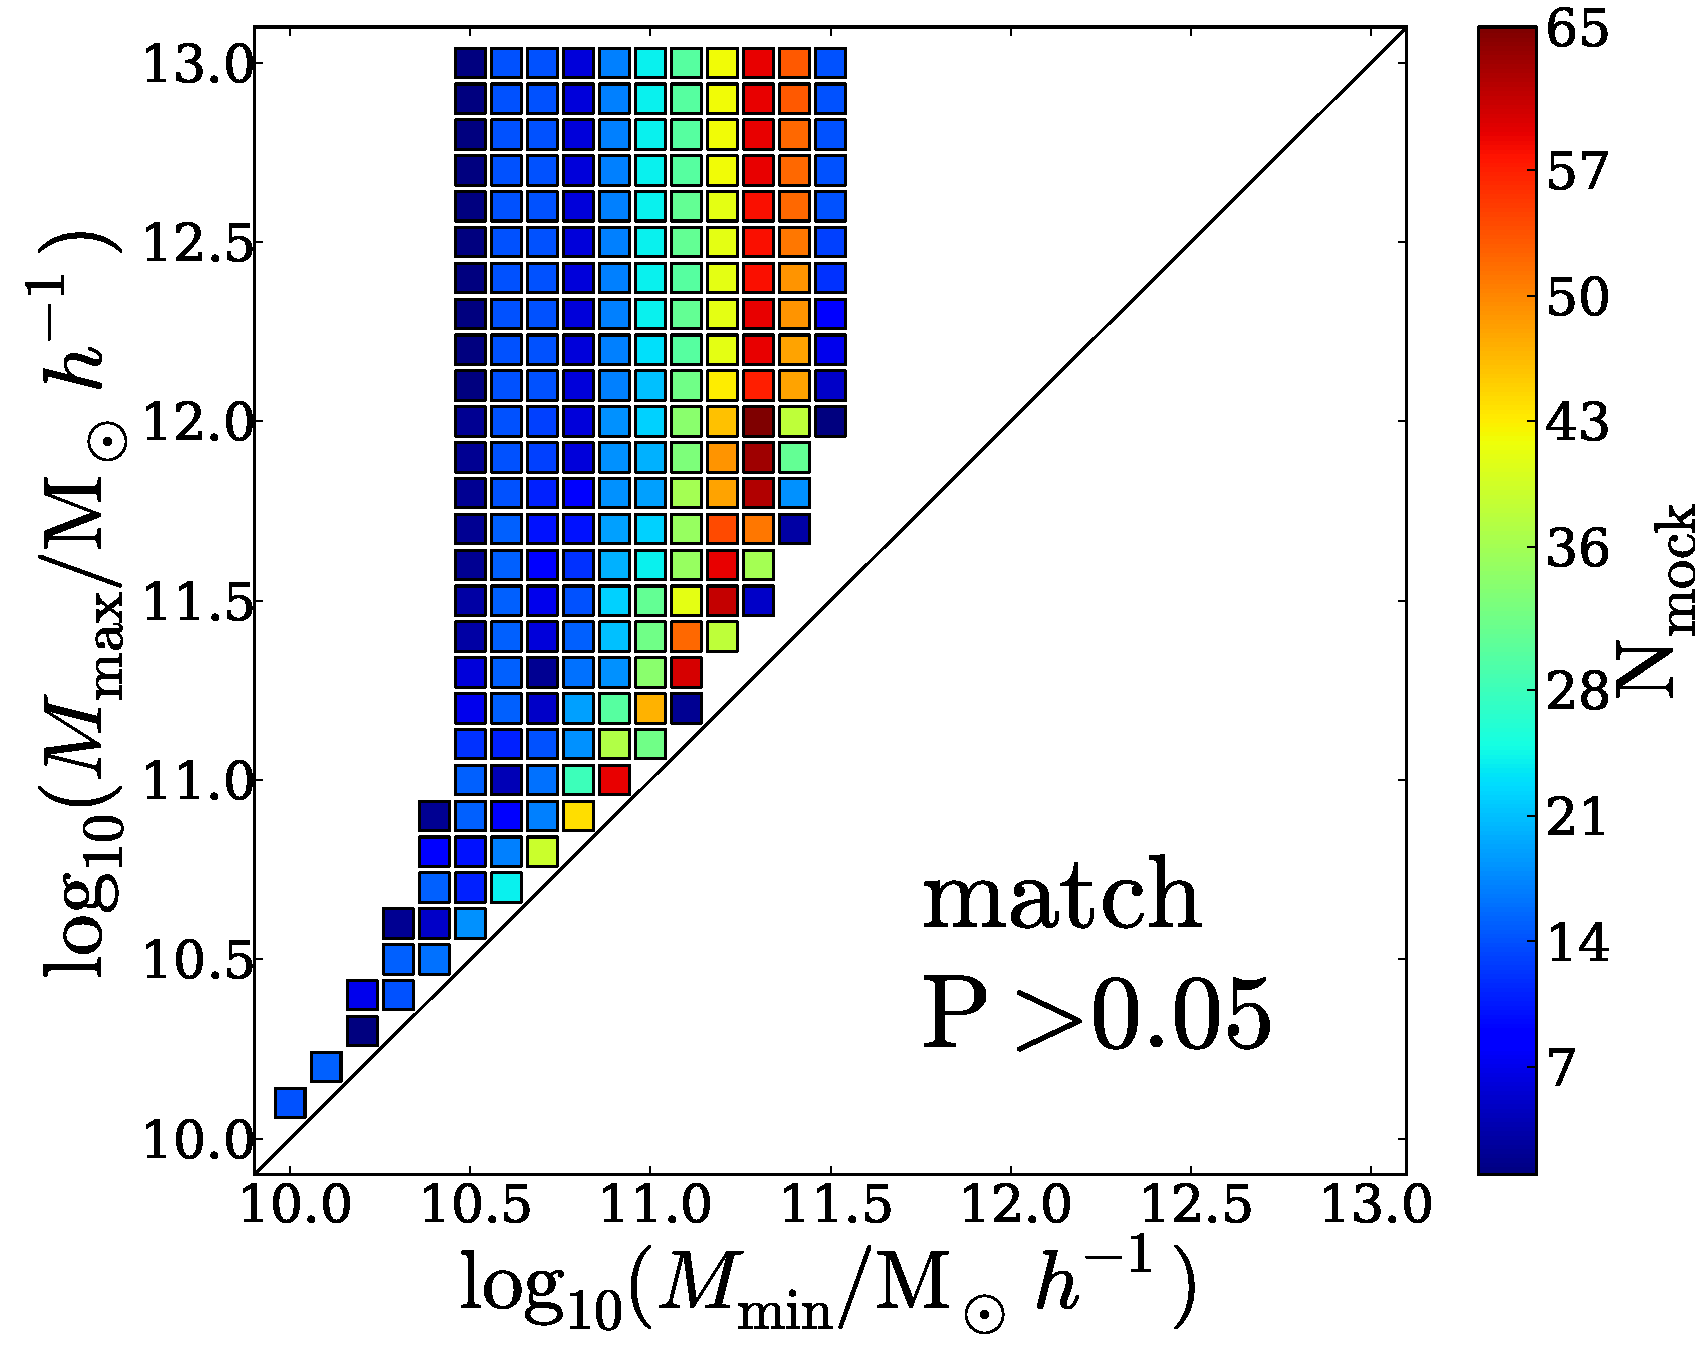
\includegraphics[width=0.46\linewidth,angle=0]{./plots/Fig2_match_P5.pdf}
\vspace{5mm}
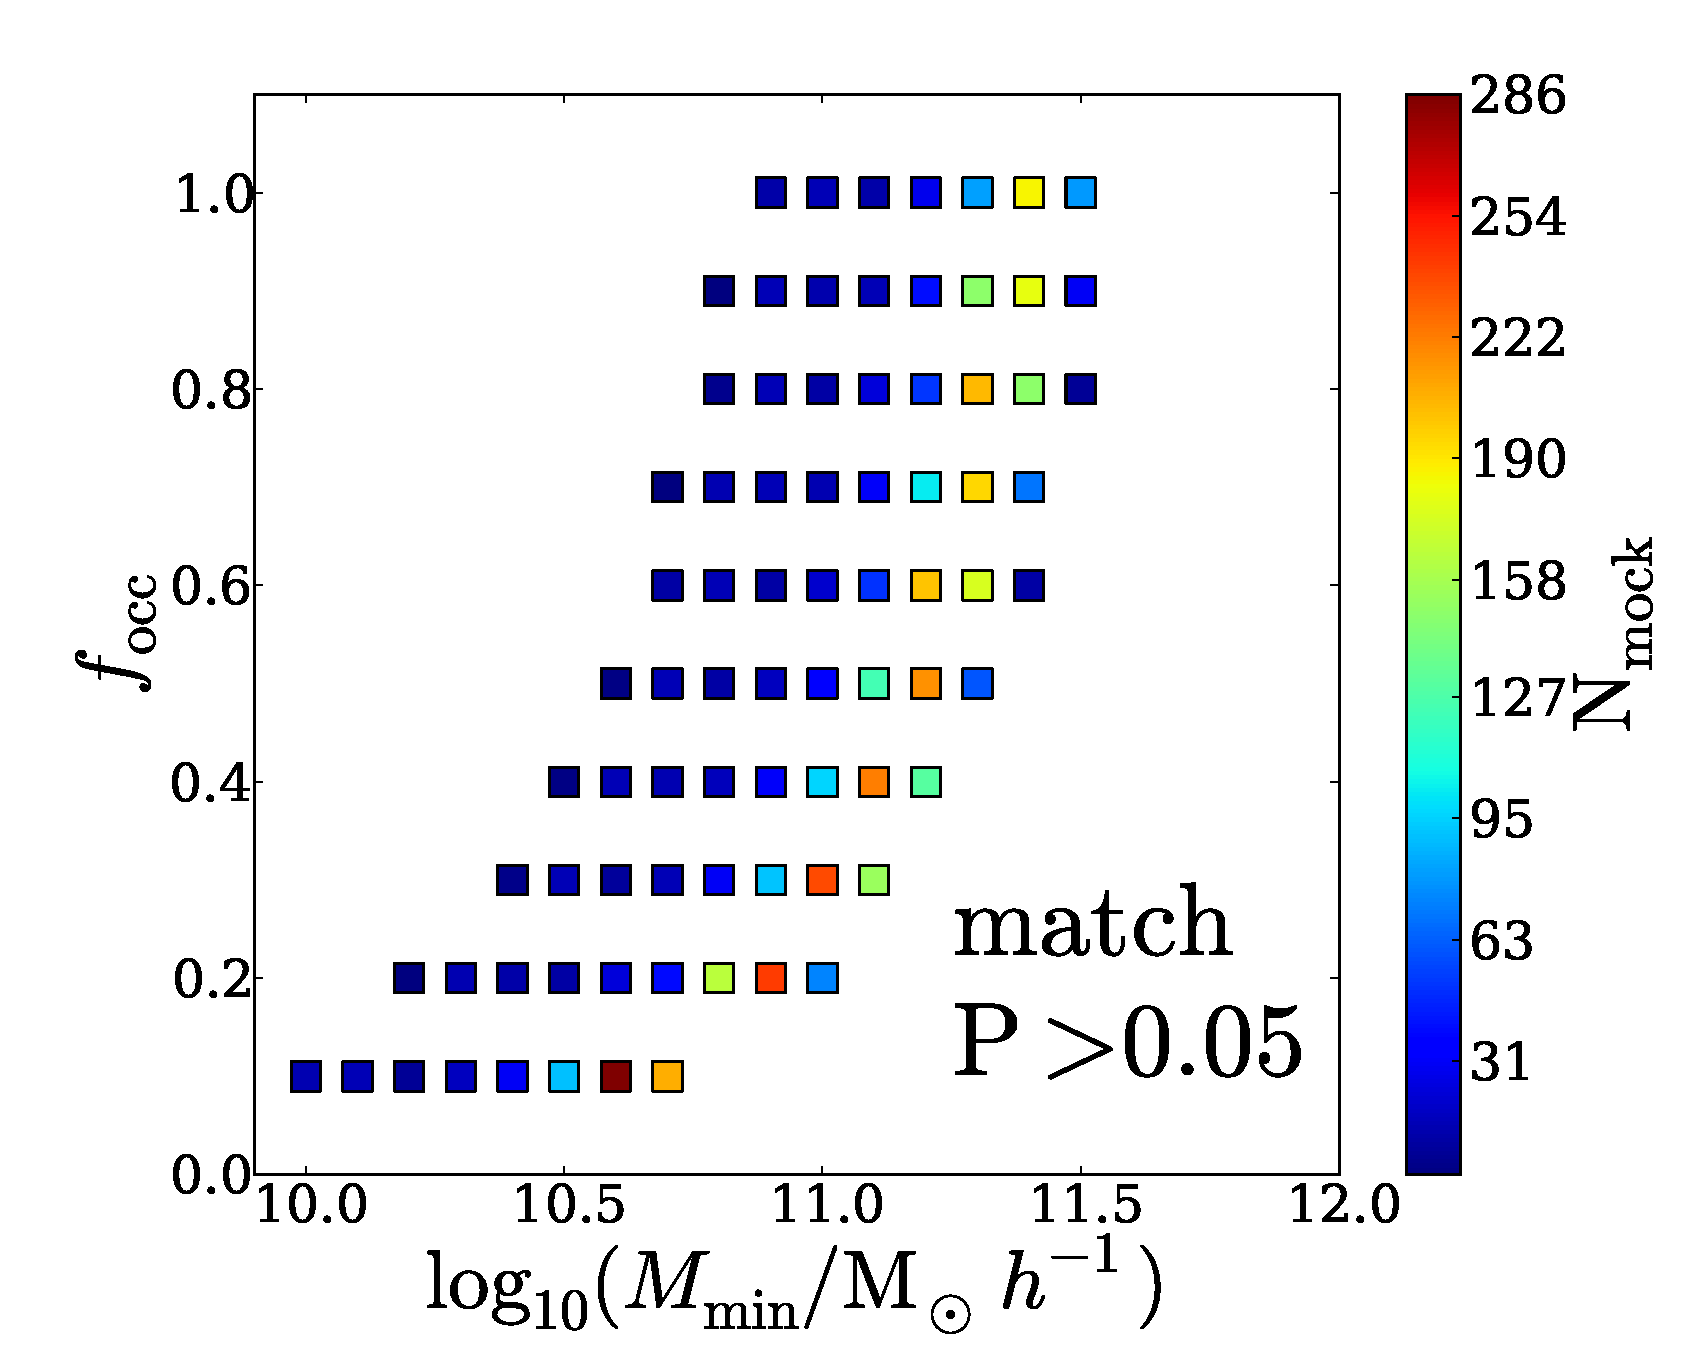
\includegraphics[width=0.49\linewidth,angle=0]{./plots/Fig3_match_P5.pdf}\\
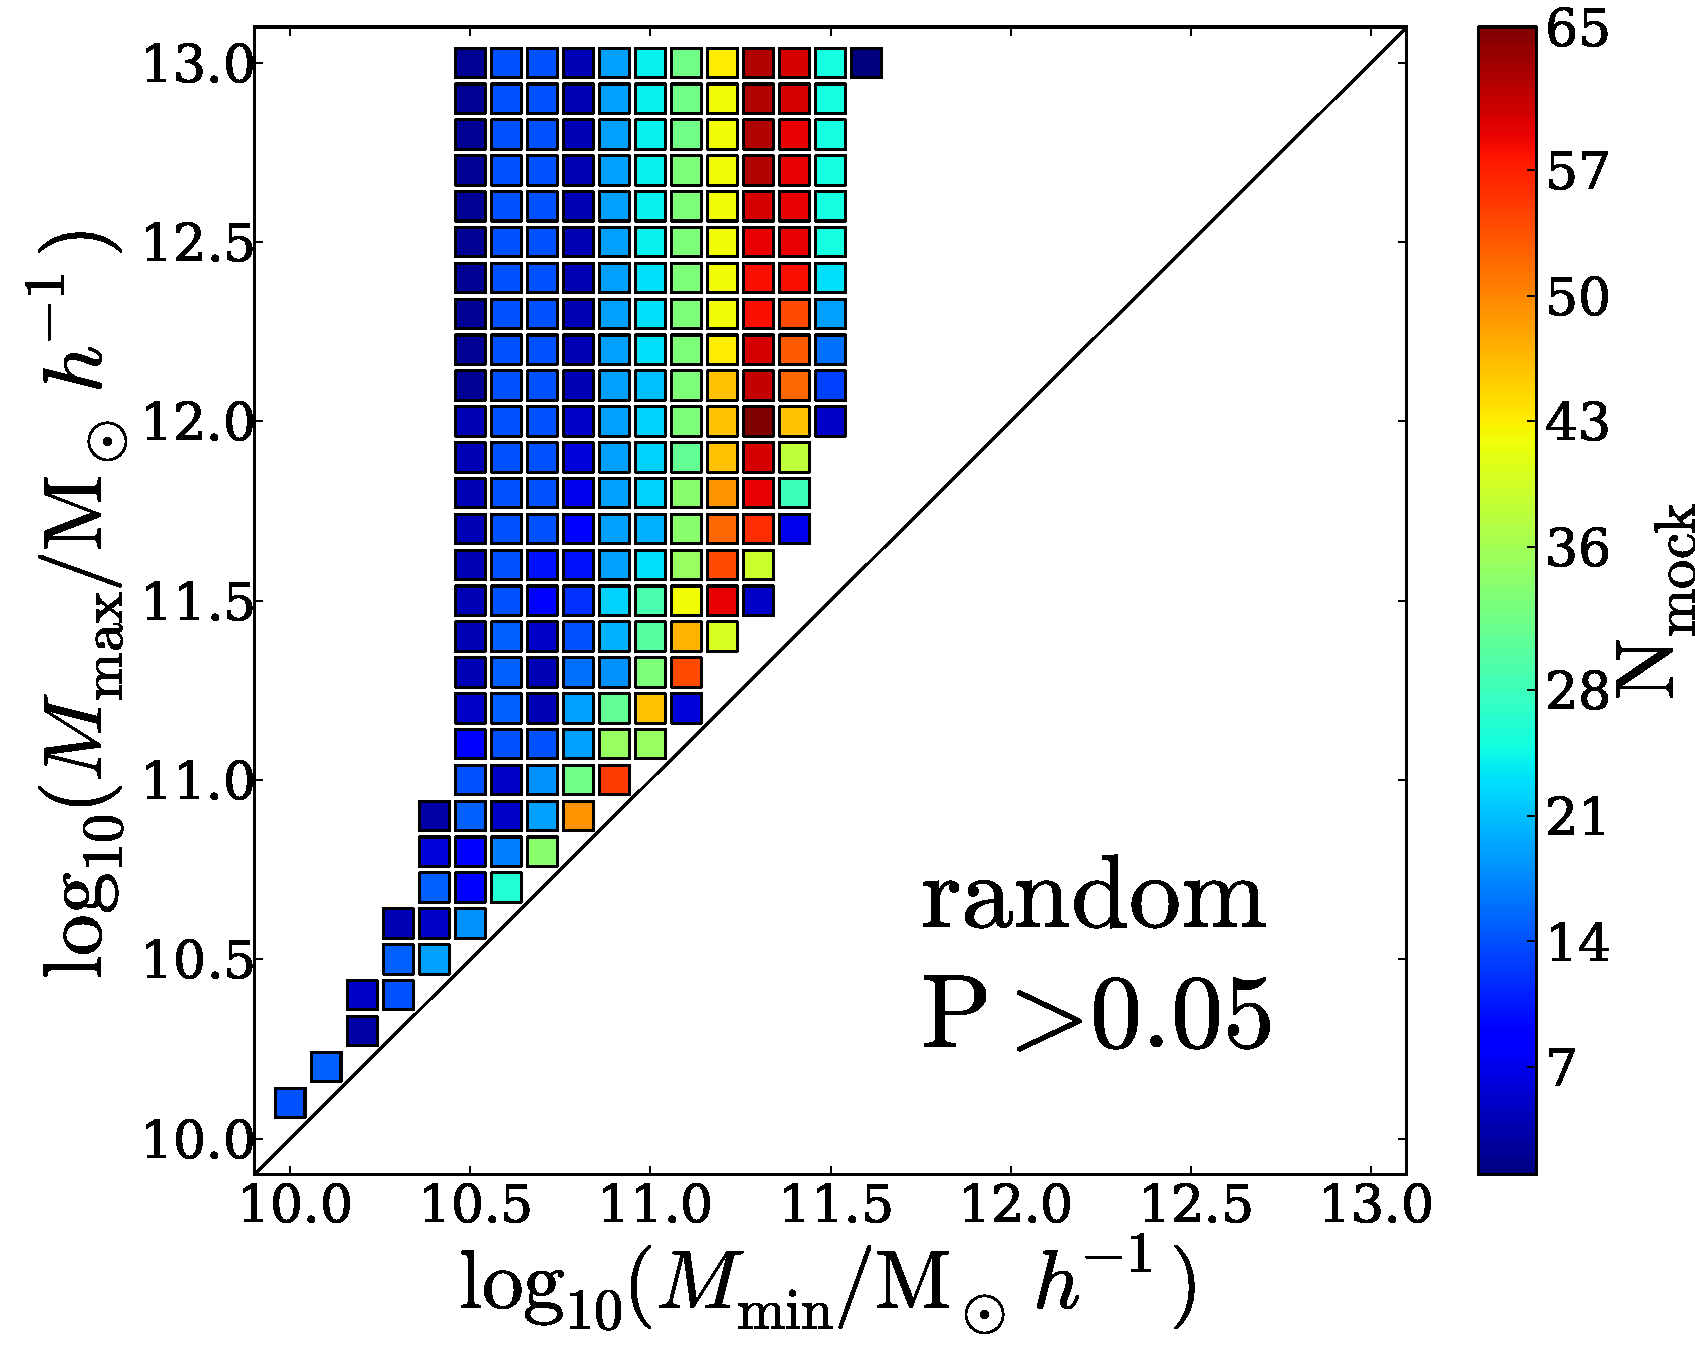
\includegraphics[width=0.46\linewidth,angle=0]{./plots/Fig2_random_P5.pdf}
\hspace{5mm}
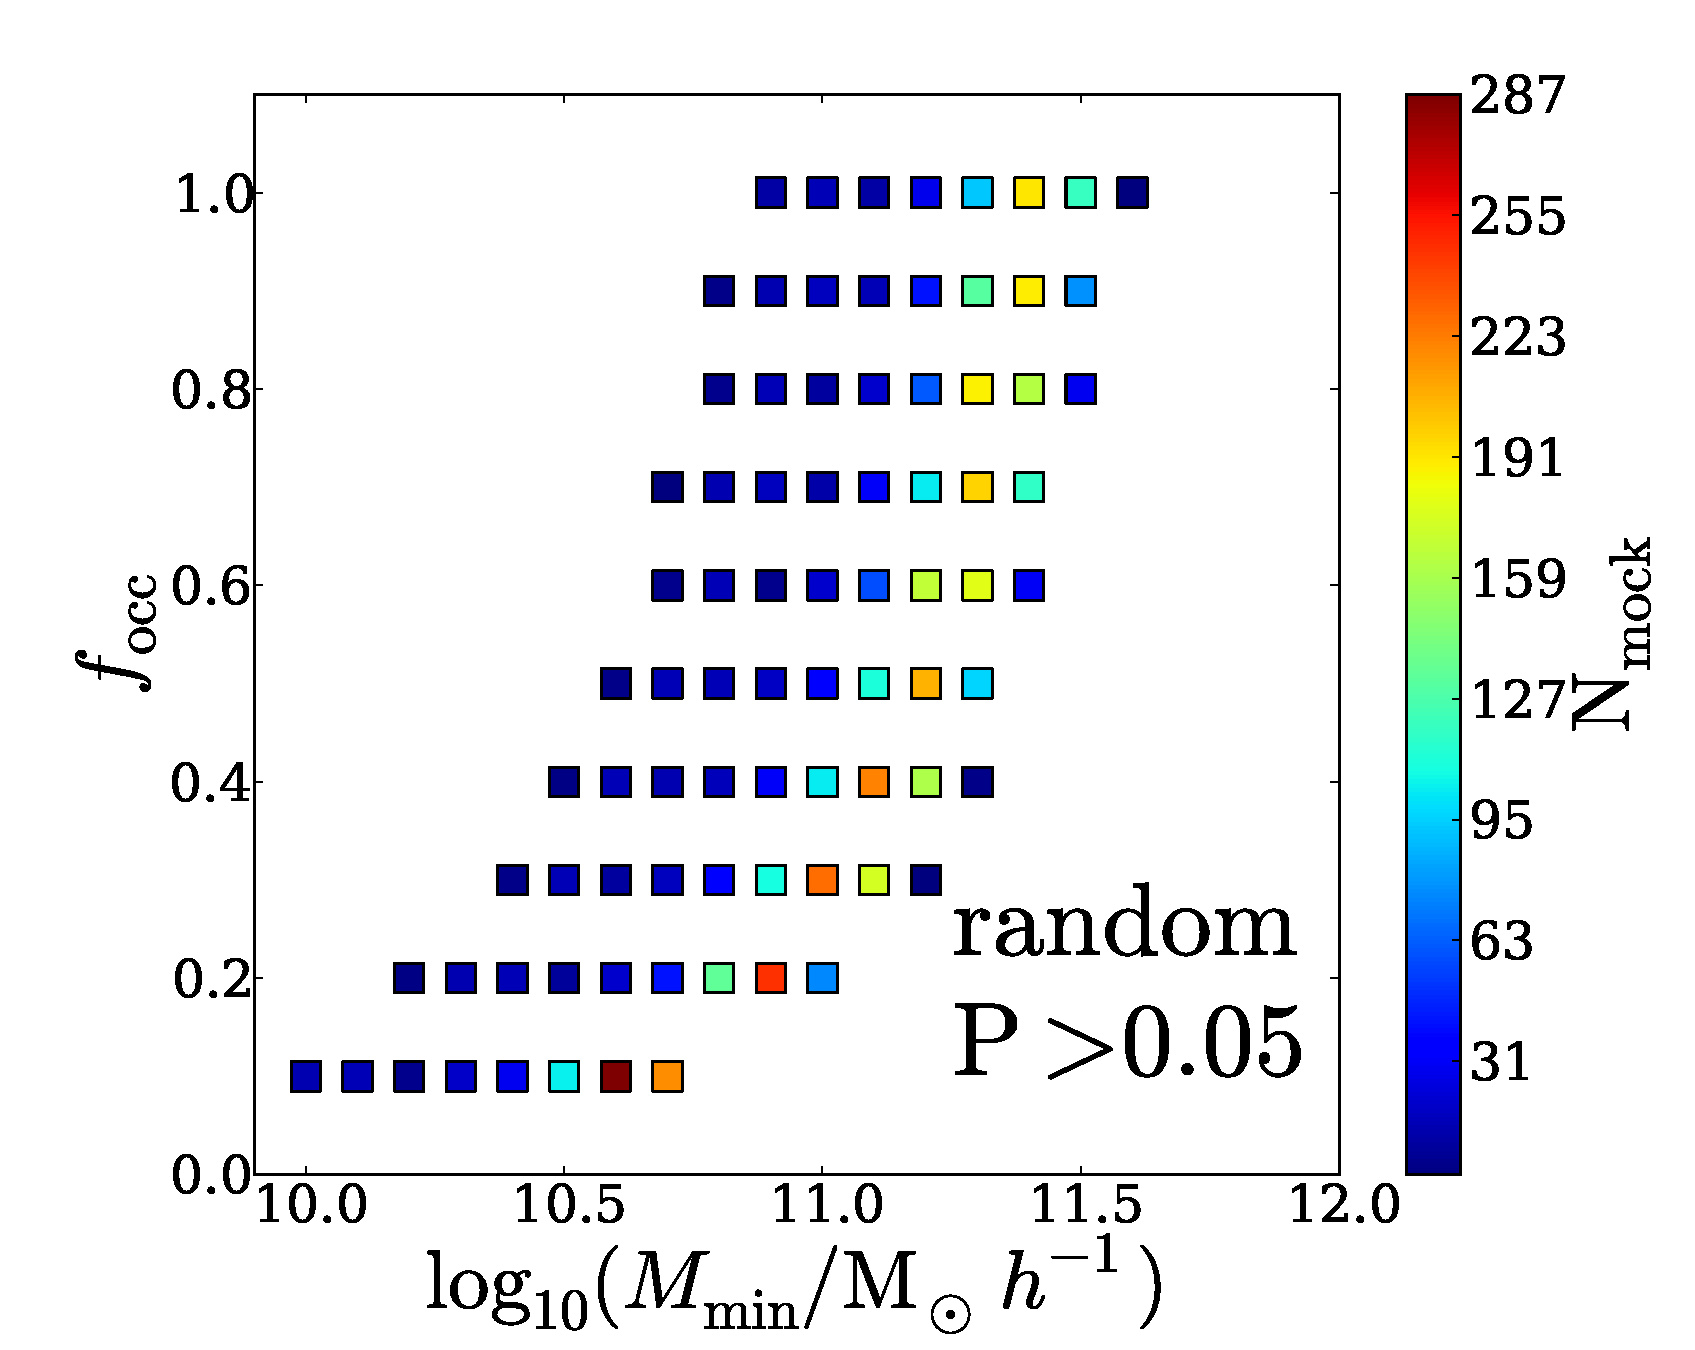
\includegraphics[width=0.49\linewidth,angle=0]{./plots/Fig3_random_P5.pdf}\\
\end{center} 
\caption{$M_{\rm min}$-$M_{\rm max}$ (left) and $M_{\rm
    min}-f_{\rm occ}$ (right) planes for all models with
  $P>0.05$ in two different ways used to construct the mock
  surveys. The color code corresponds to the number of mock surveys
  that are found to be compatible with observations in terms of the KS
  test with $P>0.05$. Only regions of parameter space with at least
  one (1) consistent mock survey are included. \label{fig:landscape}}   
\end{figure*}


Figure \ref{fig:landscape} presents regions in parameter space $M_{\rm
min}-M_{\rm max}$, $M_{\rm min}-f_{\rm occ}$ where the KS test yields
values of $P>0.05$ at least for one mock survey. For those models it
is not possible reject the hypothesis that the simulated and observed
data for the surface number density come from the same parent
distribution.

The upper (lower) panels correspond to the {\texttt match} ({\texttt
  random}) method to build the mock surveys from individual
fields. The plot shows number of mock surveys consistent
with observations. There are between $550$ to $600$ models out of the
original $9000$ models that have at least one (1) mock survey
consistent with observations. 


In Figure \ref{fig:landscale} there are three regions of parameter
space that can be clearly distinguised. The first region corresponds
to models where the minimum mass is high $\log_{10}M_{\rm min}>
11.5$. None of this models is compatible with observations as expected
from the results in the previous section. For these models the number
density of LAEs is too low. 

The second region corresponds to an intermediate range for the minimum
mass $10.5<\log_{10}M_{\rm min}<11.5$ where regardless of the value of
the maximum mass $M_{\rm max}$ it is possible to tune the occupation
fraction $f_{\rm occ}$ to bring some of the mock observations into
good agreement with observations. In this region in parameter space
one can thus find two extreme kinds of models.  One kind where the
mass interval is very narrow with sizes smaller than $<0.3$ dex (a
factor of two in mass) and others where the mass interval is very
extended, larger than $1.0$ dex, going up to the maximum halo mass
present in the simulation at that redshift. 


The third region in parameter space corresponds to $\log_{10}M_{\rm
  min}<10.5$. In this case only models with a narrow mass interval of
at most $0.5$ dex ($\log_{10}M_{\rm max}<11.0$) and low
occupation fractions $f_{\rm occ}<0.3$ are allowed. 

Without any additional information our method allows us to infer that
most of the succesful models are found in the second and third region of
parameter space where. This result was already expected from halo
abundance calculations shown in Figure \ref{fig:halos}. In the next
section we reduce the size of this region by using more stringent
constraints to define the agreement with observations and including
additional observational information onpossible values for the
occupation fraction at $z\sim 3$. 


%The raw results of our experiments yield a prefered range for
%halo masses hosting LAES bounded by a minimum mass $10.5<\log_{10}M_{\rm
%  min}<11.5$ and without any limitation on the  maximum
%mass. In this regime the average occupation fraction tends to increase
%with $M_{\rm min}$. These results discard models that were
%nevertheless disfavored from the very beginning based on the results
%of the mass functions (see Figure 1.).  


%Figure \label{figure:landscape} presents the regions in the parameter
%space $M_{\rm min}$-$M_{\rm max}$ where the KS test yields values of
%$P>0.05$. We consider that for those models it is not possible to rule out the null
%hypothesis, namely that the number density in simulated data and the observations come
%from the same parent distribution. Each panel corresponds to the three different ways of
%grouping the mock fields. In the case of the methods {\tt{Match}}
%and {\tt{Random}} the color code indicates the fraction of these 15
%mock surveys with with $P>0.1$. The third panel shows the result for
%the method {\tt{Full}}, in this case the color code correspond
%to the value maximum value of $100\times P$ for a model with those
%mass ranges.

%These results clearly distinguish three mass regimes. In the first regime, at
%high mass values, we find that LAE models with minimum mass of $M_{\rm
%  min}>10^{11.5}$\hMsun are not compatible with observations. There is
%a second regime for masses below $M_{\rm
%  min}=3\times 10^{10}$ any values for $M_{\rm min}$ and $M_{\rm max}$
%can be made compatible with observations, provided that
%$f_{\rm occ}$ is fine tuned to do it. In an intermediate mass regime,
%for minimum mass values $3\times 10^{10}\hMsun < M_{\rm min}< 3\times 10^{11}\hMsun$ only a
%limited range of models with $M_{\rm max}$ with occupation fraction
%$f_{\rm occ}\sim 1$ is able to reproduce observations. 

%In these three different mass regimes the occupation monotonically
%decreases as a function of the minimum halo mass $M_{\rm min}$. In
%Figure XXX we show this treend in three panels following the same
%correspondence as Figure XXX. From these results we interpret that the
%different mass regimes that were identified correspond to best fit
%models with $f_{\rm occ}\sim 1$, $0<f_{\rm occ}<1$ and $f_{\rm
%  occ}\sim 0$, respectively. 

%The two {\tt match} and {\tt random} methods present the highest
%number of matching mock surveys in the medium mass regime. However, it
%is important to keep in mind that not all the mock surveys for a
%sucessful model ${\mathrm M}$ present a high value $P>0.1$, only a
%modest fraction seems to be consistent with observations. This shows that the
%cosmic variance is still present on the physical scales probed by
%observations. This will be considered in more detail in the discussion
%seccion. 

%To illustrate this point, in Figure \ref{fig:mocks} we present the
%results for two mock fields for the {\tt{Match}} method for a model
%with the same parameters, but two extreme values for the KS test. 


%Conversely there are different models where the KS test yield values of
%$P\sim 1$. To illustrate the kind of success represented by these
%models, we have selected these best ones in the case of the method
%{\tt{MatchObs}}. Figure XXX shows in the main panel the spatial
%distribution of the mock surveys, the smaller panel shows the
%corresponding surface density distribution and the observational
%constraint.  

%In what follows we will focus our discussion on the mocks constructed
%with the {\tt{Match}} and {\tt{Random}} methods. 

\section{Additional Constraints}

\begin{figure*}
\begin{center}
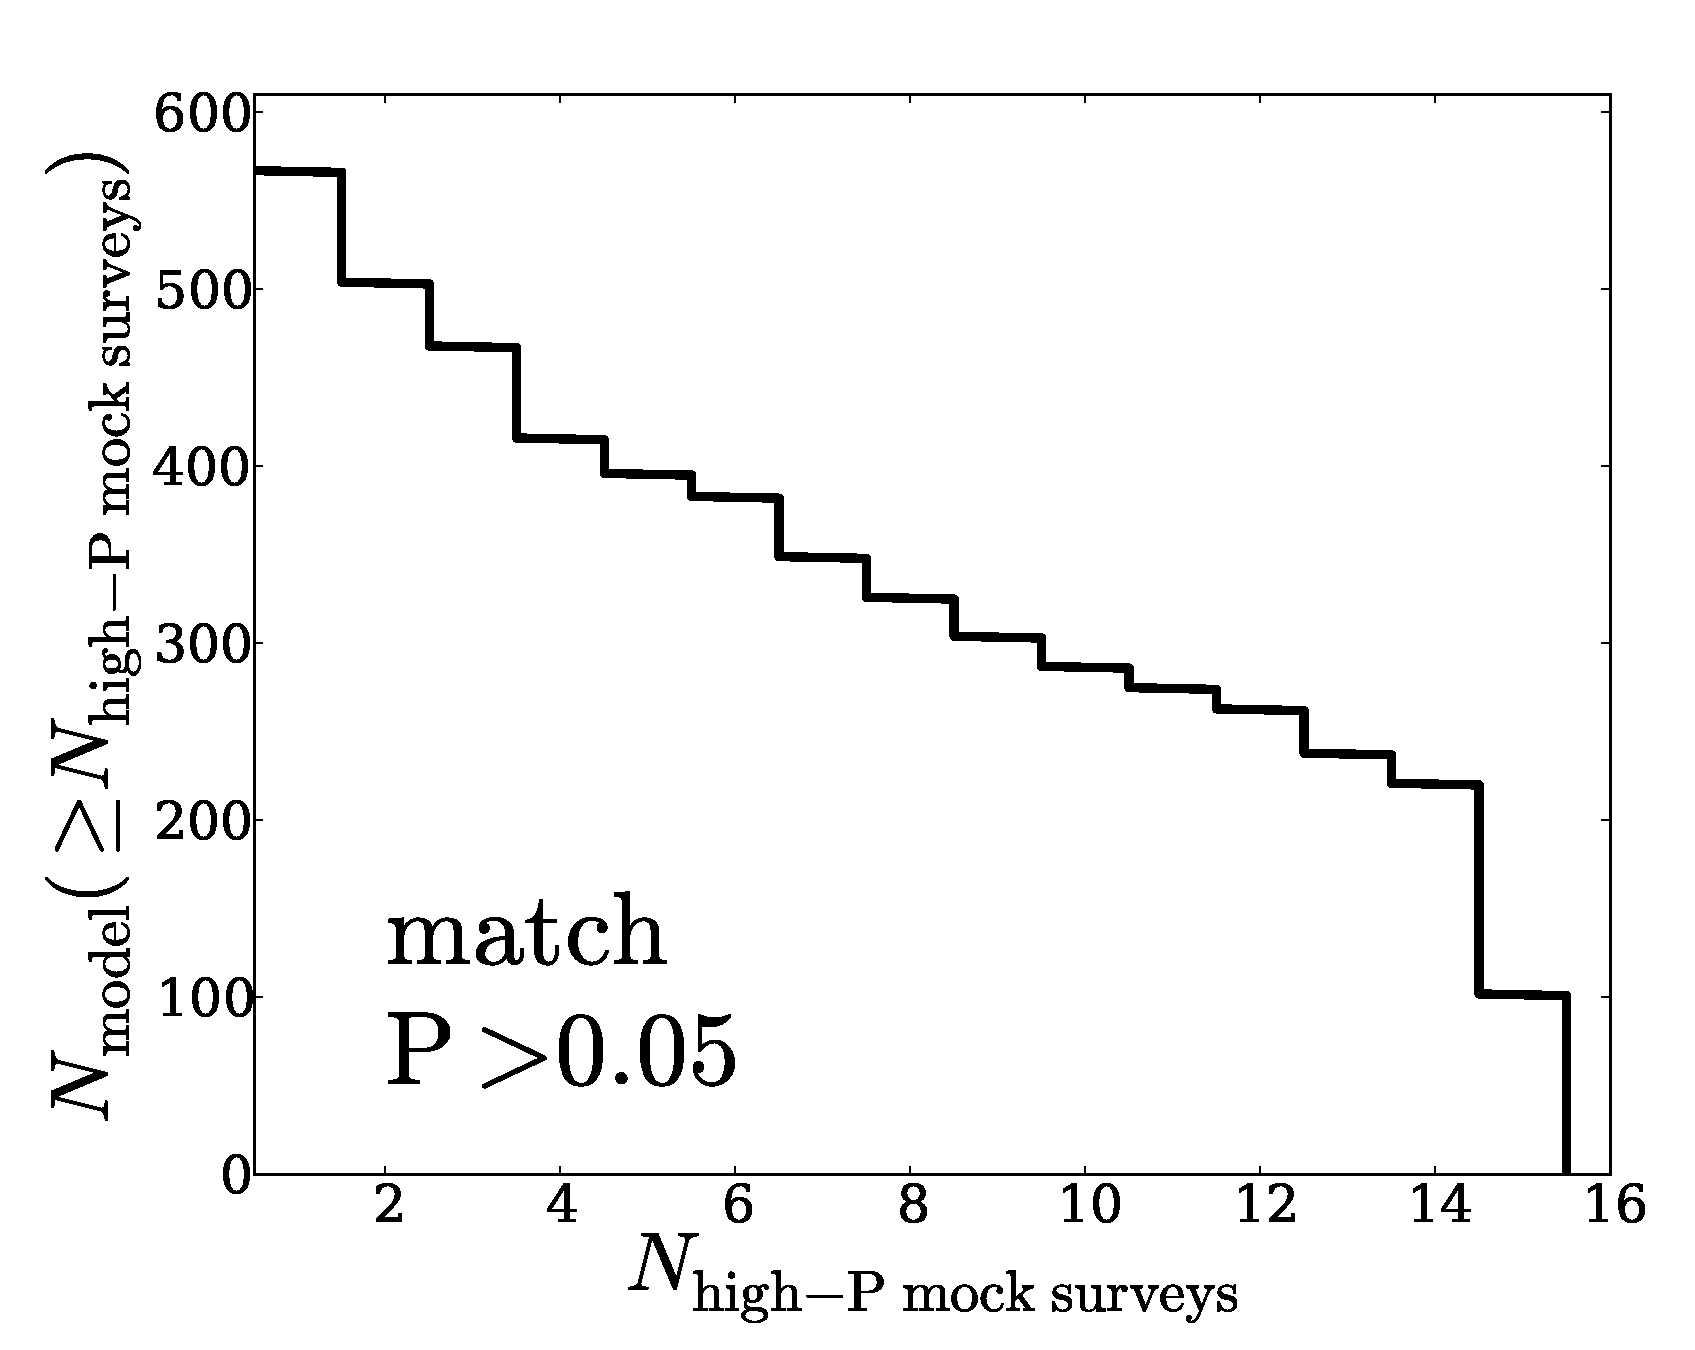
\includegraphics[width=0.46\linewidth,angle=0]{./plots/Fig4_match_P5.pdf}
\hspace{5mm}
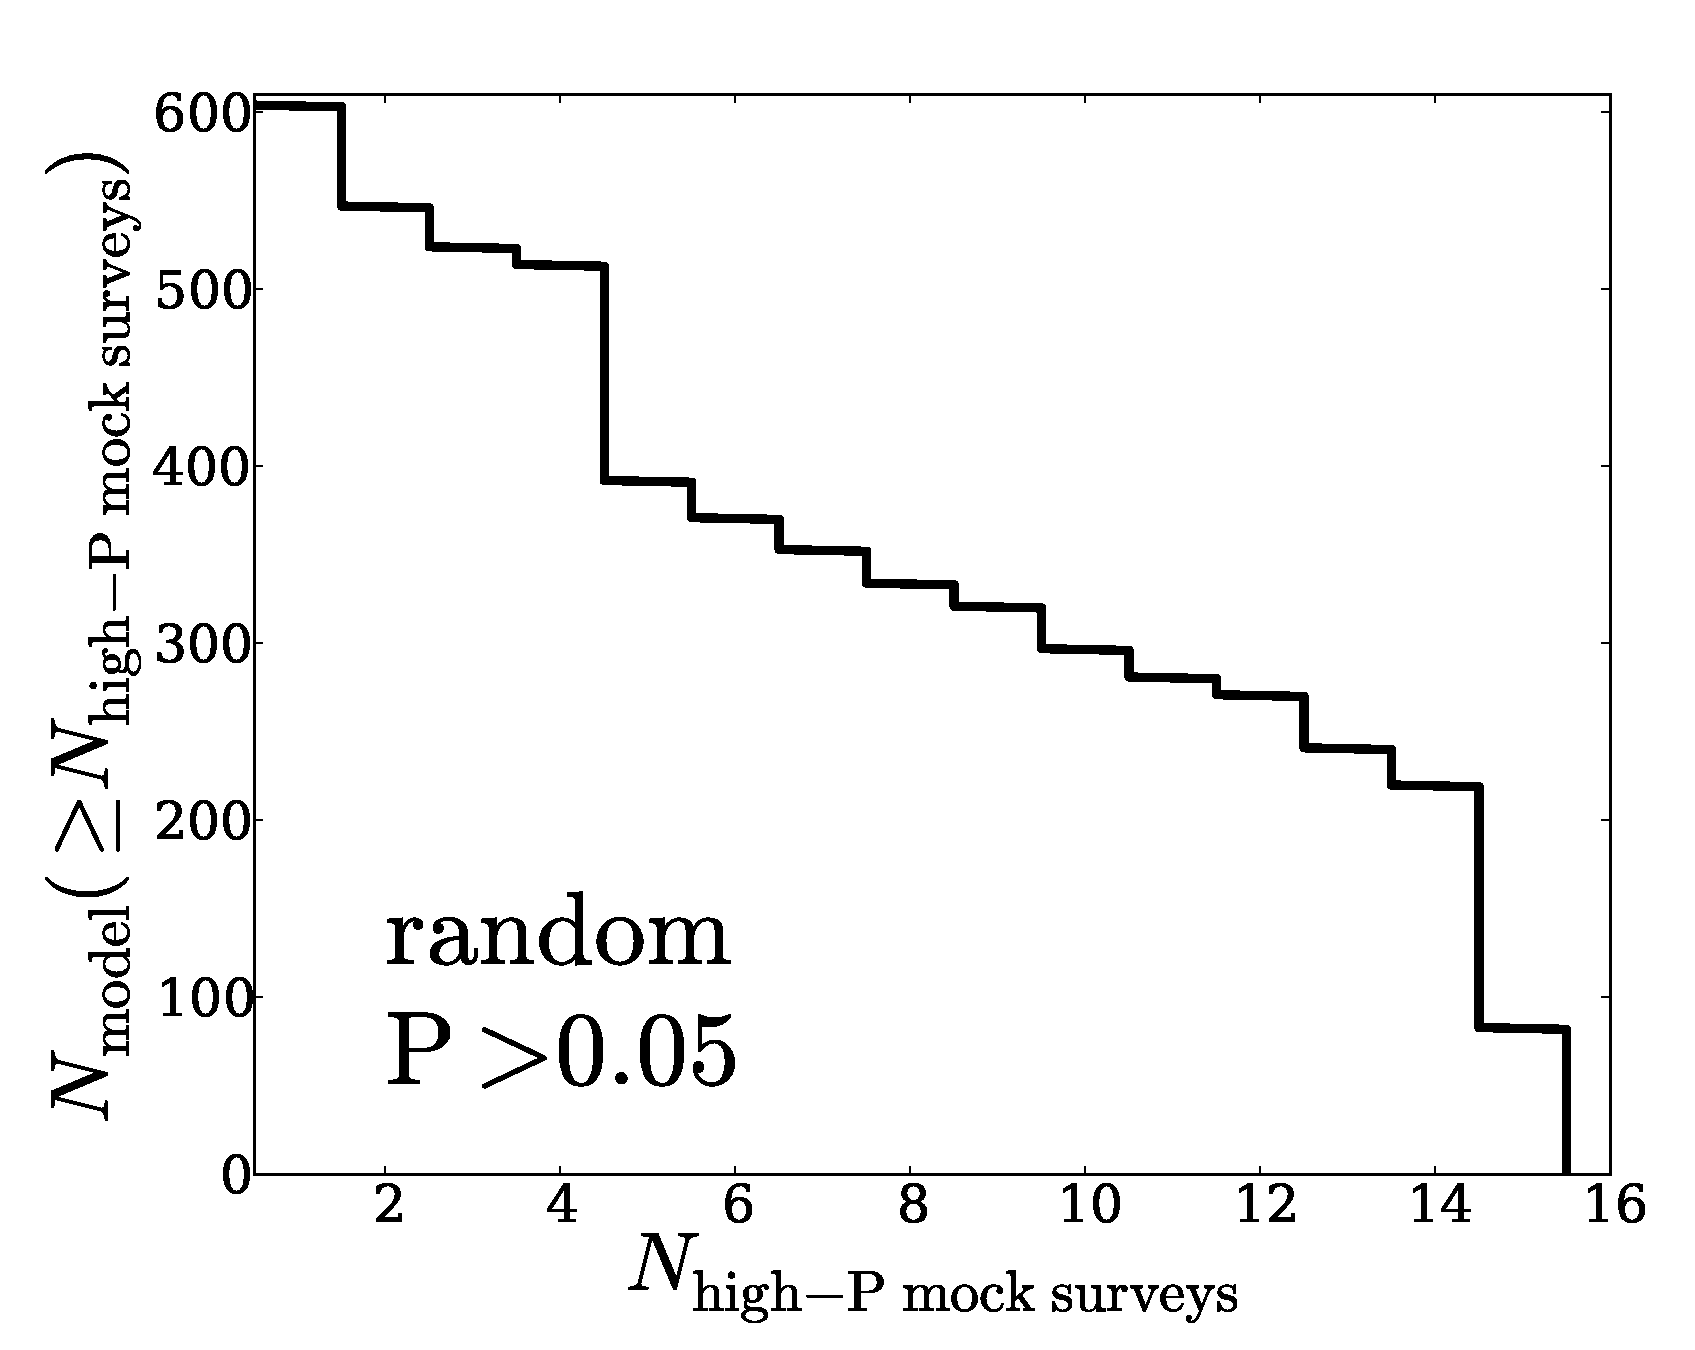
\includegraphics[width=0.46\linewidth,angle=0]{./plots/Fig4_random_P5.pdf}
\end{center} 
\caption{ Number of models with a mininium number of mock survey
  realizations that are consistent with observations.
  \label{fig:high_success_rate}.}  
\end{figure*}
 
In this section we consider two additional constraints on the models
we accept as succesul. First by taking models with the
highest possible number of mock surveys consistent with
observations. Second by including additional observational constraints
on the occupation fraction for high redshift LAEs.

%In this section we consider three different ways to impose
%tighter constraints on this mass range by making use of the results we
%have derived so far together with additional statistical and
%astrophysical constraints. In the first constraint we select the
%models where all the mock surveys present KS-test values consistent
%with observations. The second constraints uses recent observational
%results on the average occupation fraction for LAEs at high-z. The
%third exploits the information in the Angular Correlation Function
%(ACF).  

\subsection{Models with the highest success rates}

For each model ${\mathcal M}$there are 15 different mock surveys. In the
previous section we presented the models that had at least one (1)
mock survey with $P>0.05$.

Figure \ref{fig:high_success_rate} shows the number of models
that have at least $N_{\rm high-P}$ mocks with $P>0.05$ for the {\texttt
  match} and {\texttt random} methods.  This shows that there are
here are between $80$ to $100$ models with all the 15 realizations with
$P>0.05$. This a reduction of a factor of $\sim 6$ with repect to the
total number of mocks with at least one consistent mock. 
%Here we focuse on the latter models. 
%The best models
%represent $\sim 15\%$ of the number of initially considered good
%models. 

Figure \ref{fig:restriction_mock} presents the locii of these models
in the parameter space $M_{\rm min}-M_{\rm max}$ and $M_{\rm
  min}-f_{\rm occ}$ for the {\texttt match} method, the results for
the {\texttt random} method are similar. In this case the models with
$\log_{10}M_{\rm min}< 11.7$ are greatly reduced. This corresponds to
the regions in the parameter space in Figure \ref{fig:landscape} that
already had a low number of consistent mock surveys. From the right
panel in Figure \ref{fig:restriction_mock} one can see that there is
not a strong selection effect on the occupation fraction $f_{\rm
  occ}$. 

\subsection{Additional  Constraints on the Occupation Fraction}

We impose an additional restriction using the observational results
by \cite{Hayes2010}. They constrained the value of $f_{\rm
  occ}$ at $z=2.2$ to be $f_{\rm occ}=0.10$. This estimation was based
on blind surveys of the H$\alpha$ and Lyman $\alpha$ line with the European Southern
Observatorio (ESO) Very Large Telescope (VLT). Using corrections by
extinction to obtain an estimate for the intrinsic H$\alpha$
luminosity, and using values for the theoretical expectation of the
ratio Lyman$\alpha$/H$\alpha$ they derive an bulk escape fraction for
the Lyman$\alpha$ radiation of $f_{\rm esc}=(5.3\pm 3.8)\%$ or $f_{\rm
esc}=(10.7\pm 2.8)\%$ if a different dust correction is used. The
authors show that the luminosity function for LAEs at $z=2.2$ is
consistent with the escape fraction being constant for every galaxy
regardless of its luminosity. From this results they derive that
almost $90\%$ of the star forming galaxies emit insufficient
Lyman $\alpha$ to be detected, effectively setting the occupation
fraction to be $f_{\rm occ}=0.10$. For the cosmological parameters
used in this \documentname the age of the universe between $z=3.1$ and
$z=2.2$ has changed by $\sim 1$ Gyr. We assume that the physical
conditions that determine the escape fraction $f_{\rm esc}$ and the
occupation fraction $f_{\rm  occ}$ remain similar over that time
scale.

We limit the occupation fraction to
be in the range 
%further pick models that have an occupation fract
$f_{\rm
  occ}\leq 0.2$ to allow for some flexibility on the time evolution
and the uncertainty in the dust correction used to infer the escape fraction. 
%Considering an occupation fraction $f_{\rm occ}=0.20$
%another $39$This constraint help us to
%select $\sim 10\%$ of theoriginal models that were considered as
%consistent with observations in the previous section. 
Figure  \ref{fig:restriction_mock_and_f_occ}  shows the prefered
models in the planes $M_{\rm min}-M_{\rm  max}$ and $M_{\rm
  min}-f_{\rm occ}$ for the {\tt match} and {\tt   random} methods.
With this additional constraint between $35$ to $40$ models are
consistent with observations, this represents a factor of $\sim 2$
reduction. All the models with $\log_{10}M_{\rm min}\geq 11.0$ are now
excluded and the best models are now clustered around a narrow region
in parameter space. The list for the model parameters is in the
Appendix in Table \ref{table:models_match}. 


%In terms of the constraints done in the previous sub-section, we find
%that the models in this region of parameter space have an average
%number of XX mock catalogs consistent with observations. 

\begin{figure*}
\begin{center}
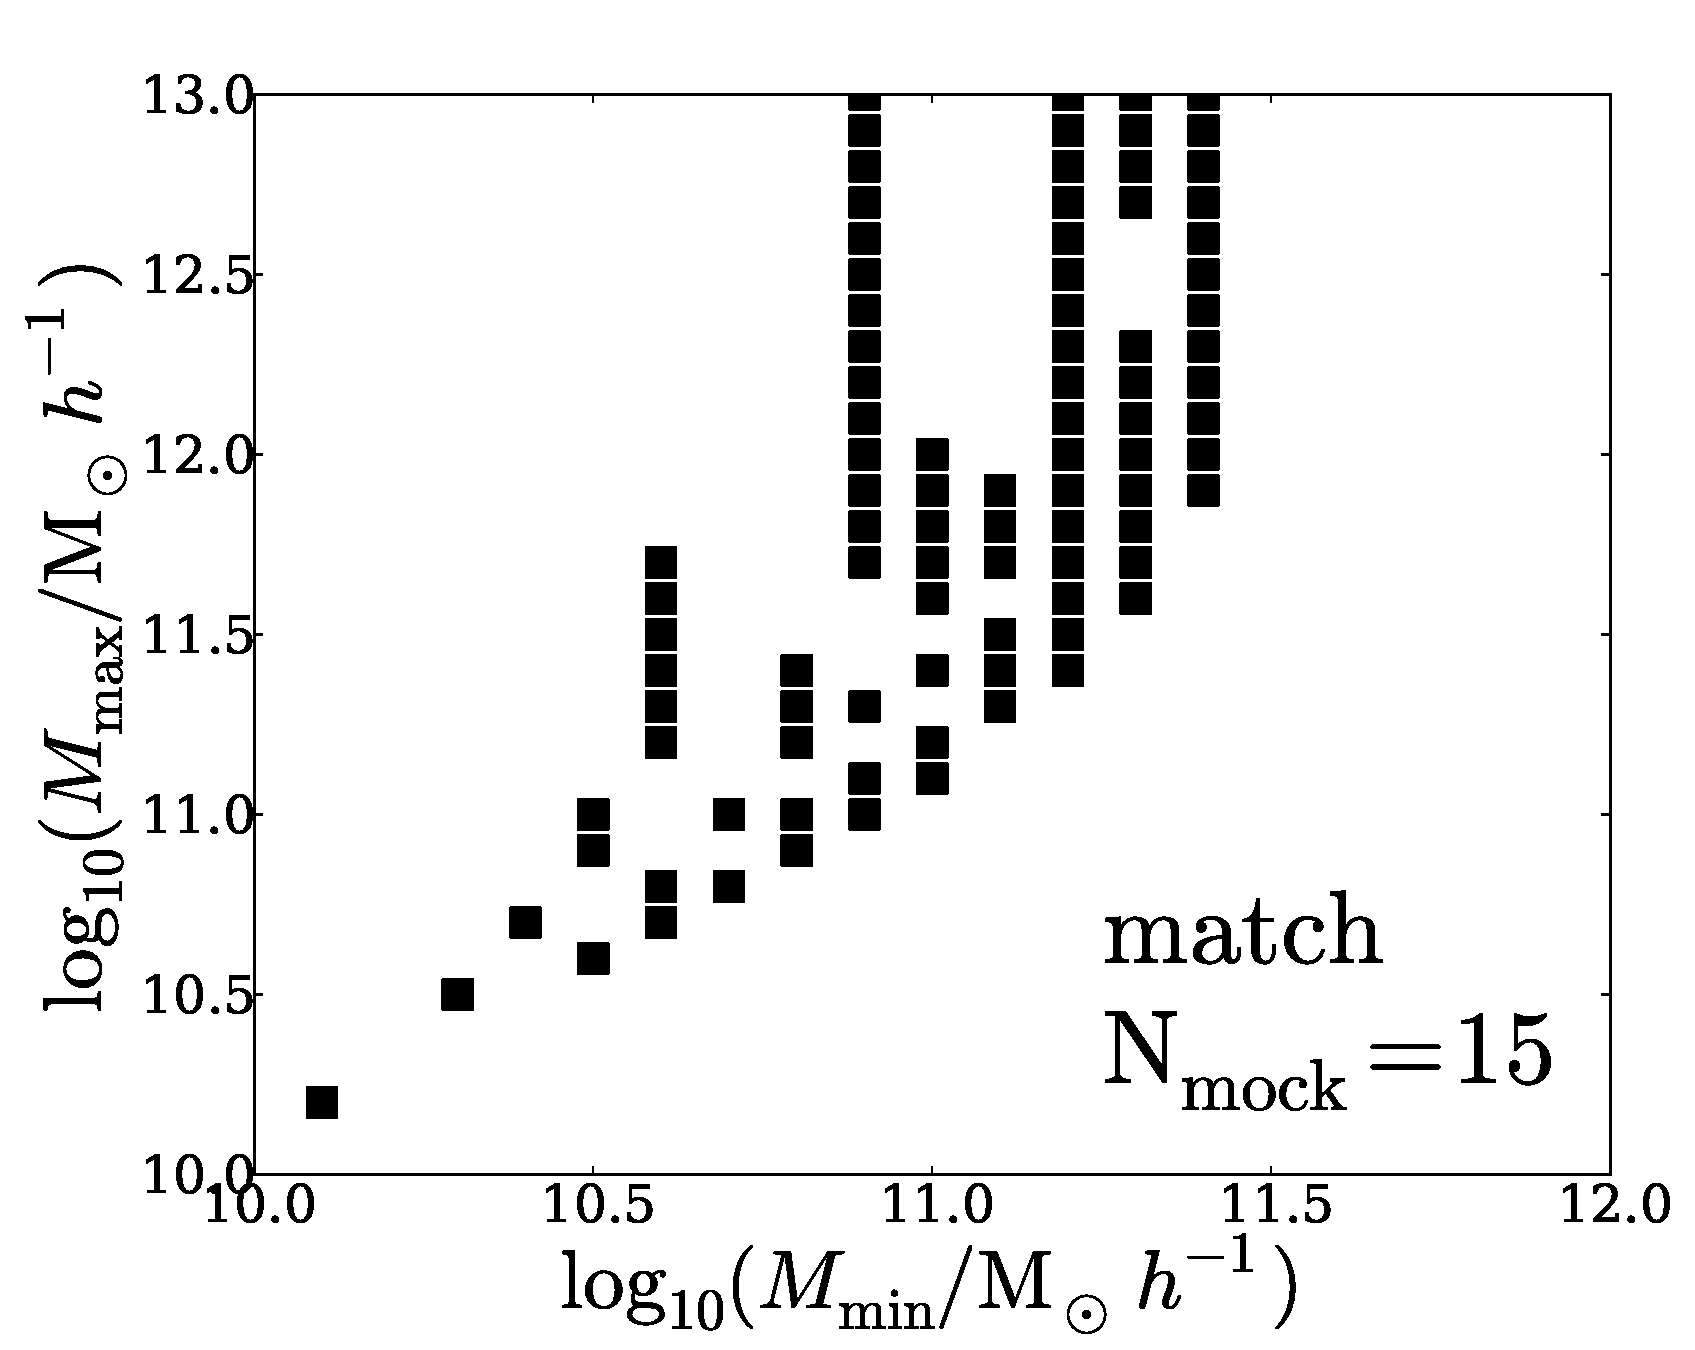
\includegraphics[width=0.46\linewidth,angle=0]{./plots/Fig5_match_mass_mock.pdf}
\hspace{5mm}
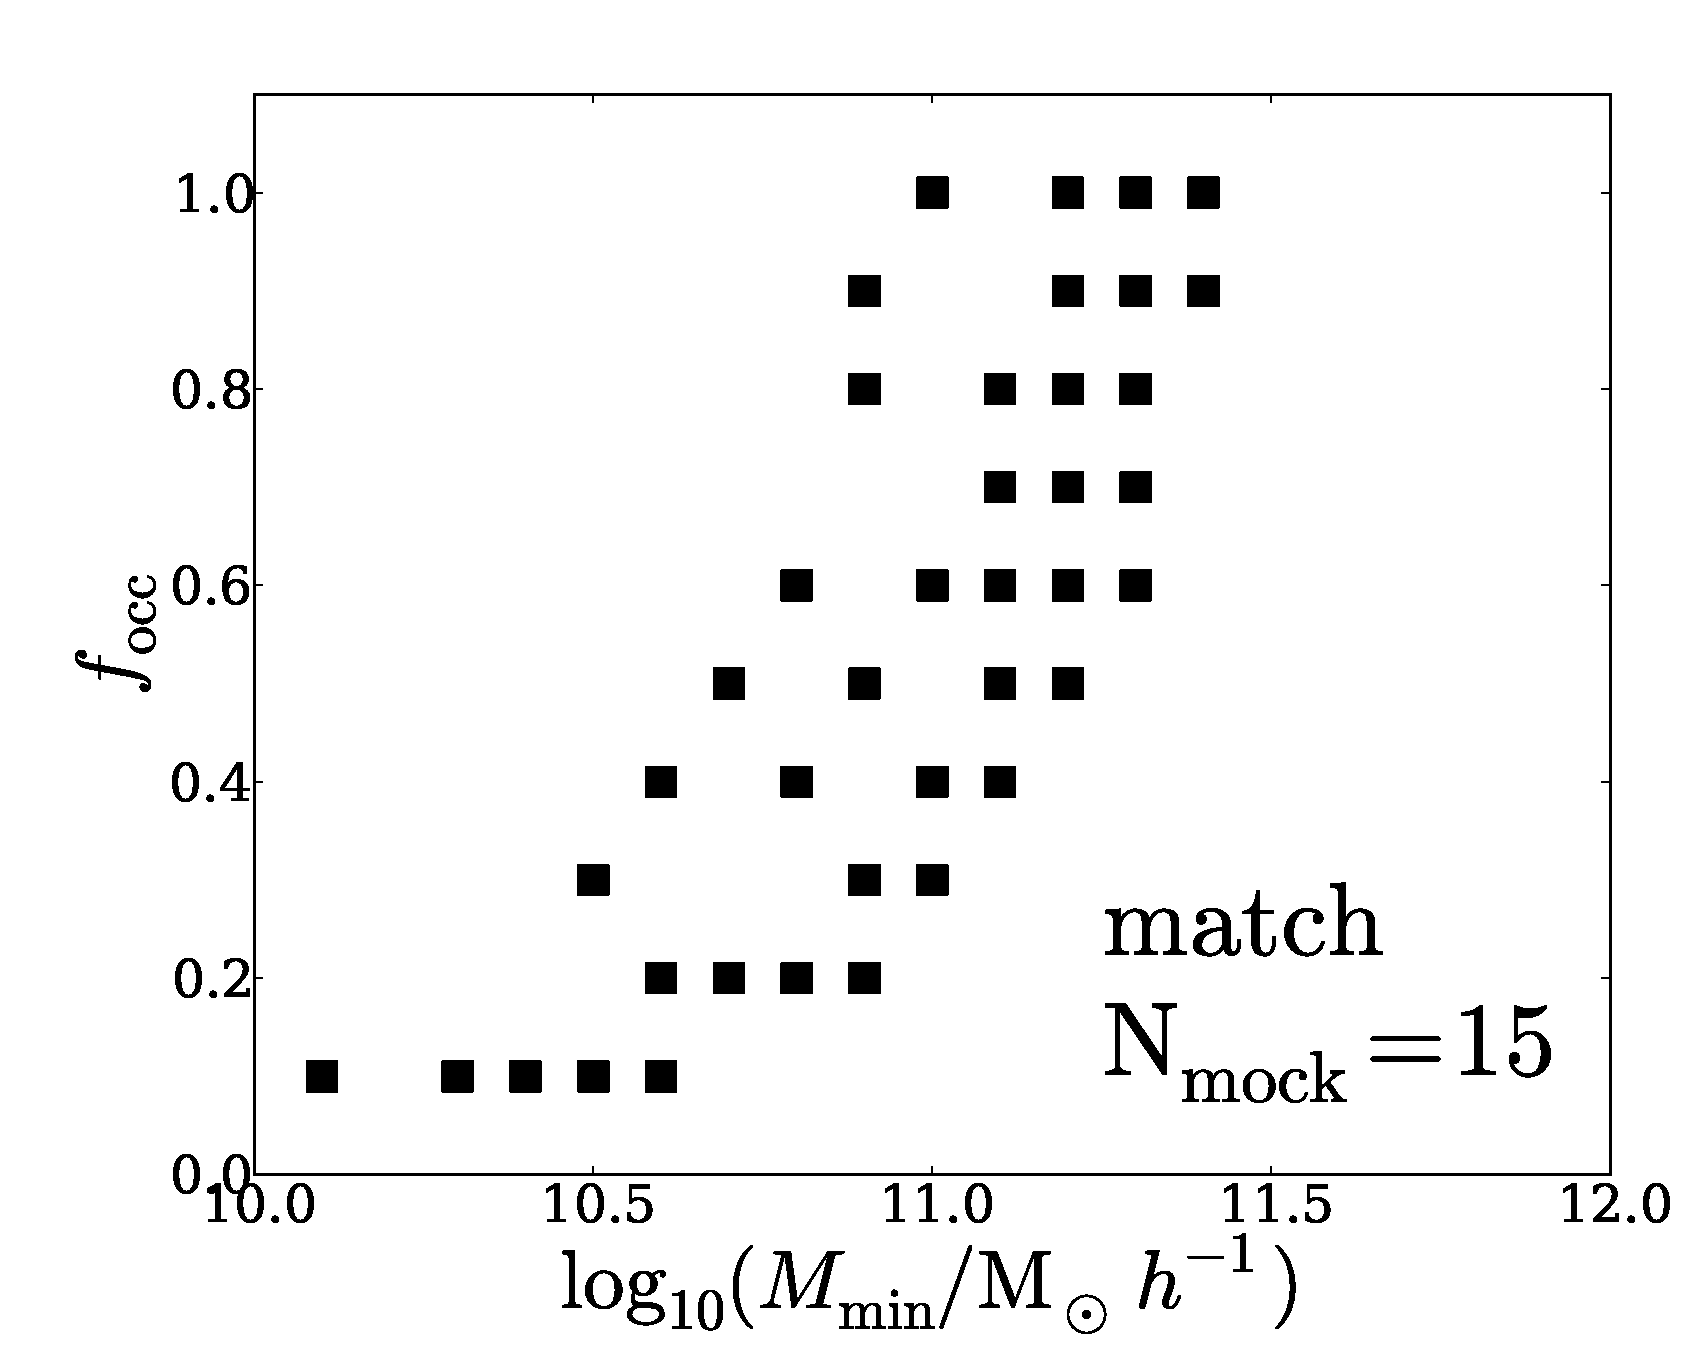
\includegraphics[width=0.46\linewidth,angle=0]{./plots/Fig5_match_f_occ_mock.pdf}
\end{center} 
\caption{Favored regions in parameter space when the constraints on
  the maximal number of consistent mocks is imposed. The results for
  the {\texttt random} methodology (not shown here) are very similar to the ones
  presented here for the {\texttt match} method.
  \label{fig:restriction_mock}}  
\end{figure*}


\begin{figure*}
\begin{center}
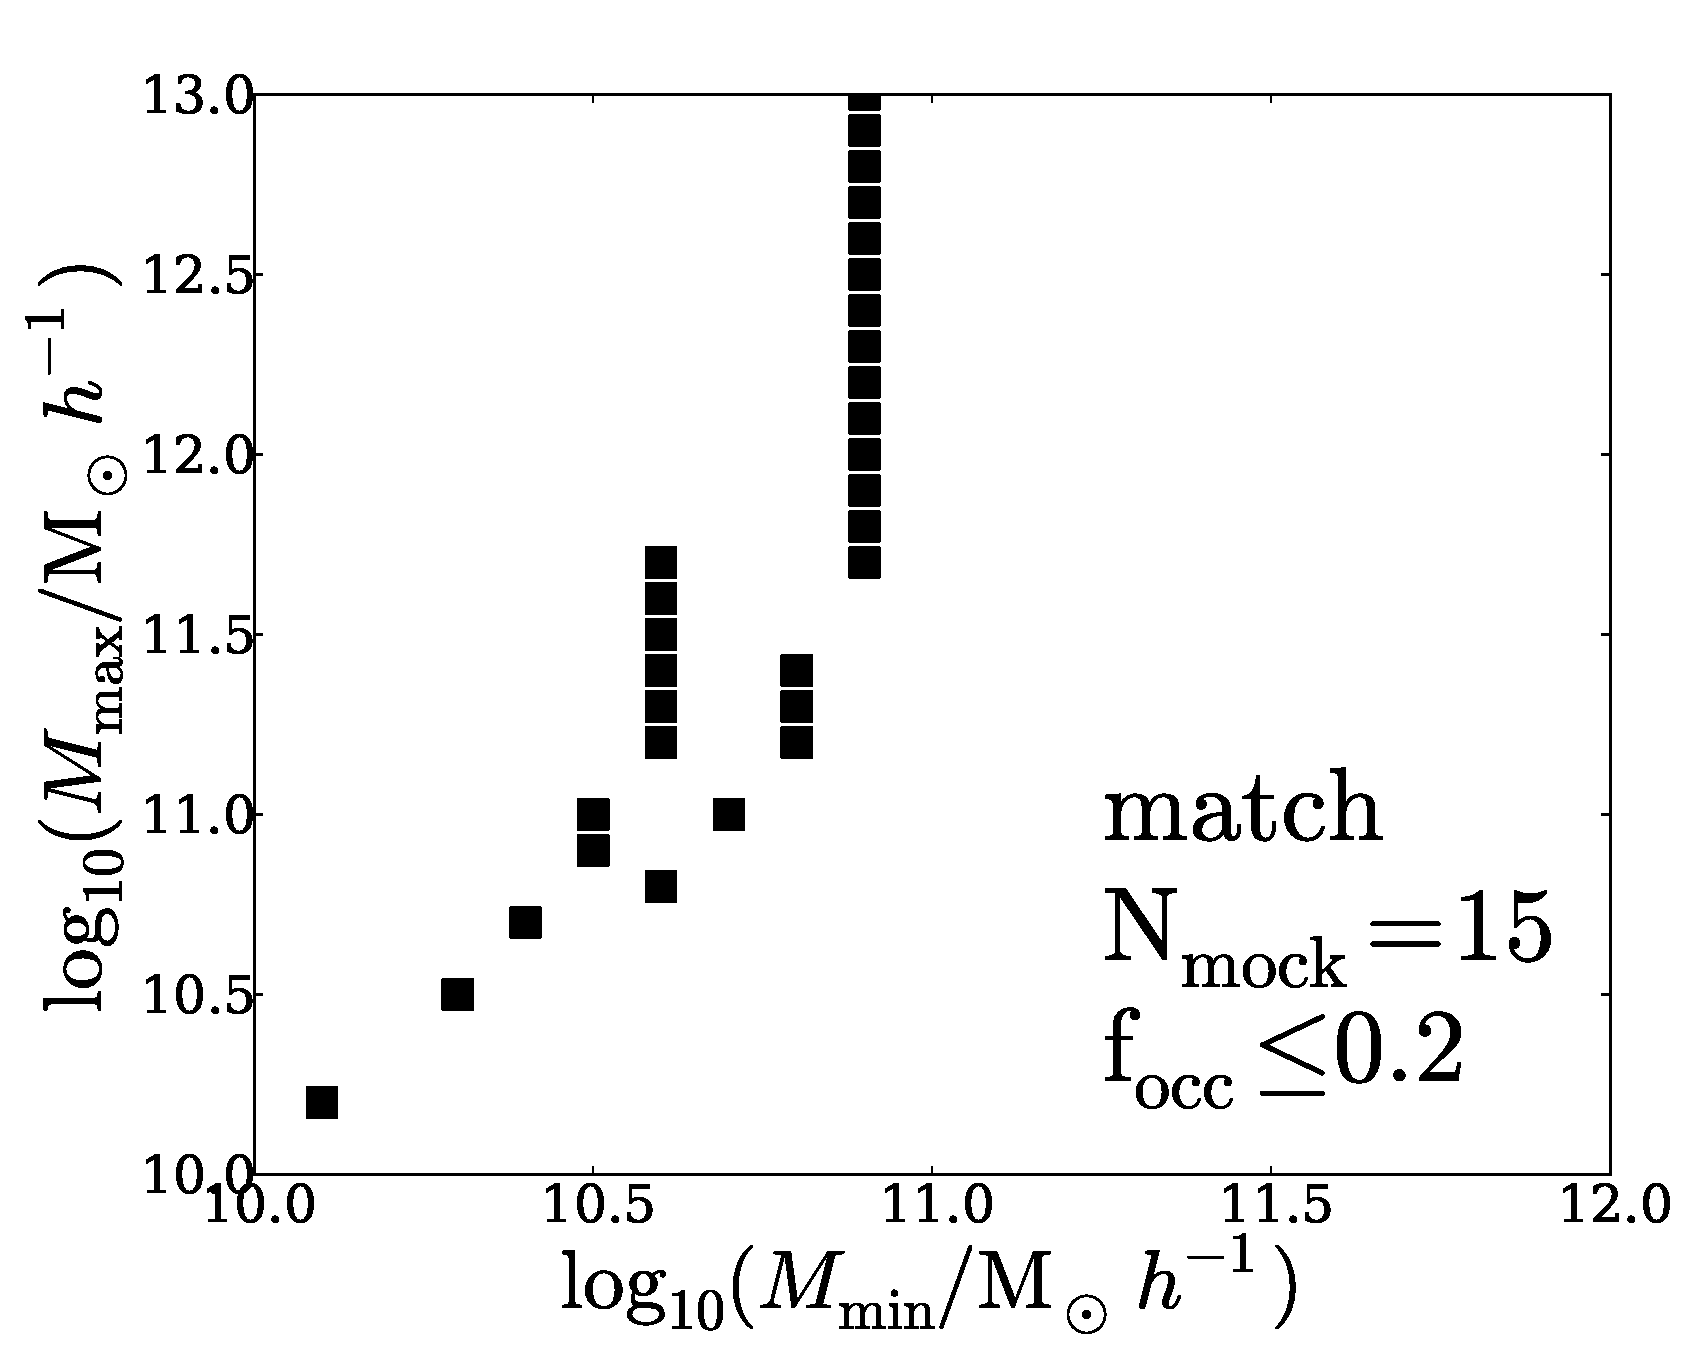
\includegraphics[width=0.46\linewidth,angle=0]{./plots/Fig5_match_mass_mock_and_f_occ.pdf}
\hspace{5mm}
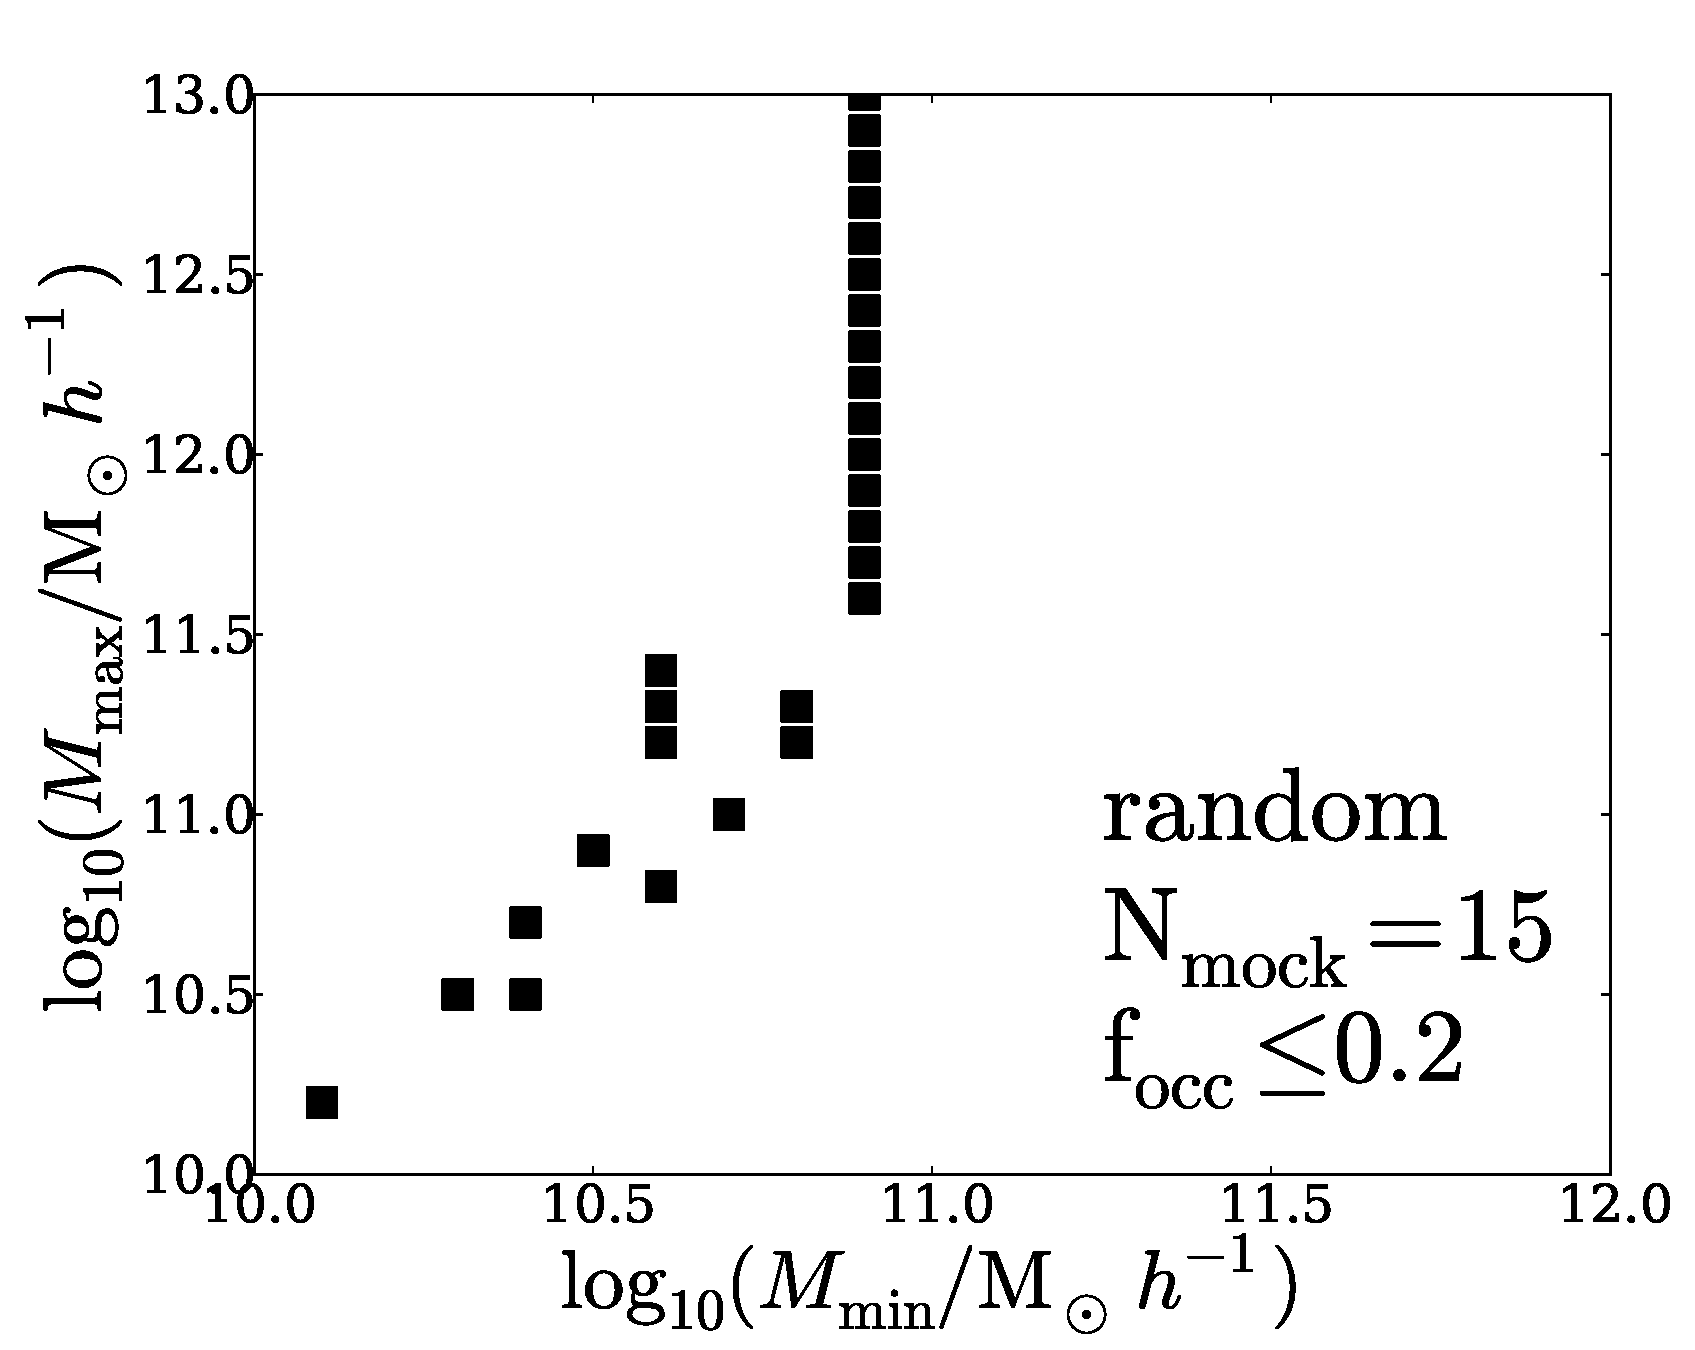
\includegraphics[width=0.46\linewidth,angle=0]{./plots/Fig5_random_mass_mock_and_f_occ.pdf}
\end{center} 
\caption{Best models when both the constraints on the maximal number
  of  consistent mocks and the occupation  fraction $f_{\rm occ}\leq
  0.2$ are included.  \label{fig:restriction_mock_and_f_occ}}   
\end{figure*}



\section{Results for the Angular Correlation Function}

We calculate the mean angular correlation function (ACF) only for the
models that showed that all of the 15 mock surveys are consistent
at the $P>0.05$ level with observations. The ACF is computed only the
denseset subfield in all the 15 mock surveys corresponding to the
SSA22 region. These results are compared against the observations
reported by Hayashino et al in 2004 over the same region, which were
also performed on the densest field.   

Figure \ref{figure:correlation_match} (match) and Figure
\ref{figure:correlation_random} (random) present such comparison.  The
error bars in these figures represent the standard deviation of the
ACF over all the sub-fields.  In general, we observe that the standard
deviation of the computed ACF in the subfields increases with
$M_{min}$ following the same trend as in Figure
\ref{figure:laes_dist}, as a direct consequence of cosmic variance.  


The comparison between the simulated and observed ACFs is also done using a
$R^2$ statistic which includes the information on measurement uncertainties

\begin{equation}
R^{2} = \sum_{\theta_i} \frac{(\xi_{\rm obs}(\theta_i) - \xi_{\rm
    sim}(\theta_i))^2}{\sigma_{\rm obs}^2(\theta_i) + \sigma_{\rm
    sim}^2({\theta_i})}, 
\end{equation}

where the sum is done over all the angle values $\theta_i$ where the
ACF has been computed. In Figure XX we plot the integrated
distributions for this $R^{2}$ statistics 

Given that the ACF reported by Hayashino et al en 2004 is taken over
the densest  field oserved in the SSA22 region by  Yamada et el in
2012 it is expected that the predicted ACF in the SSA22 region should
reproduce this observation. In the  left panel of figure
\ref{figure:correlation_match} we can see the predicted ACFs  an their
corresponding standard deviation over the seven fields that mock the
SSA22  region. It can be seen that the model with $M_min=10.6$ seems
to better reproduce the  Hayashino's ACF and that the corresponding
field is in fact an overdense field in the SSA22 region covered by
Yamada et al. 

From these tests we conclude that the ACF on small fields does not
provide additional constraints to further select models for halos
hosting LAEs. The reason is that cosmic variance is large and the
statistical uncertainties on the ACF render almost any model
compatible with the observational constraints. 

We also present the ACF in the case of the full SSA22
region which has been homogeneously observed by \citep{Yamada2012}. To
this date the observational ACF has not been reported in the
litereature, therefore our calculations can be considered as
predictions. 

In Figure X we present the results for the models. The full list of
these correlation functions can be found in the the data repository
for this paper in \verb"github". 

We also present the results for the angular correlation function in
therms of the correlation lenght obtained by fitting the following
function

\begin{equation}
\xi(r) = \left(\frac{r}{r_{0}}\right)^{-\gamma}
\end{equation}

The results are shown in Figure in a $r_{0}-\gamma$ plane where the
average and standard deviation for each mock are shown in comparison
with the result derived from observations. 


%\begin{figure*}
%\begin{center}
%\includegraphics[width=0.46\linewidth,angle=0]{./plots/match_large_correlation_%selected_models.pdf}
%\hspace{5mm}
%\includegraphics[width=0.46\linewidth,angle=0]{./plots/match_full_correlation_s%elected_models.pdf}
%\end{center} f
%\caption{ mean ACFs   and their correponding standard deviation (error
%  bars)  of some selected models in different mass ranges over the 7
%  subfields  f the SSA22 field (left) and the entire 12 field sample
%  (rigth) using thematch
%  configuration. \label{figure:correlation_match} }  
%  \end{figure*}

%\begin{figure*}
%\begin{center}
%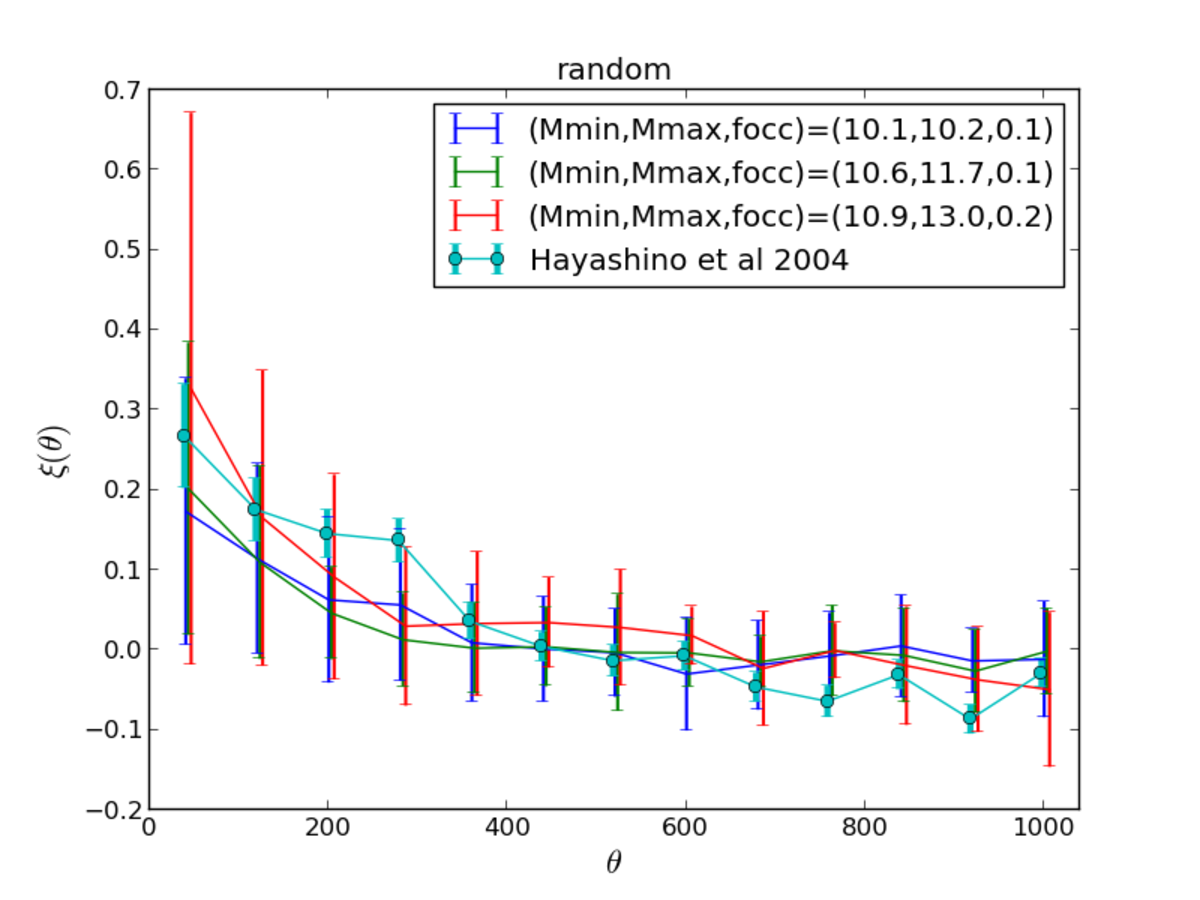
\includegraphics[width=0.46\linewidth,angle=0]{./plots/random_large_correlation_selected_models.pdf}
%\hspace{5mm}
%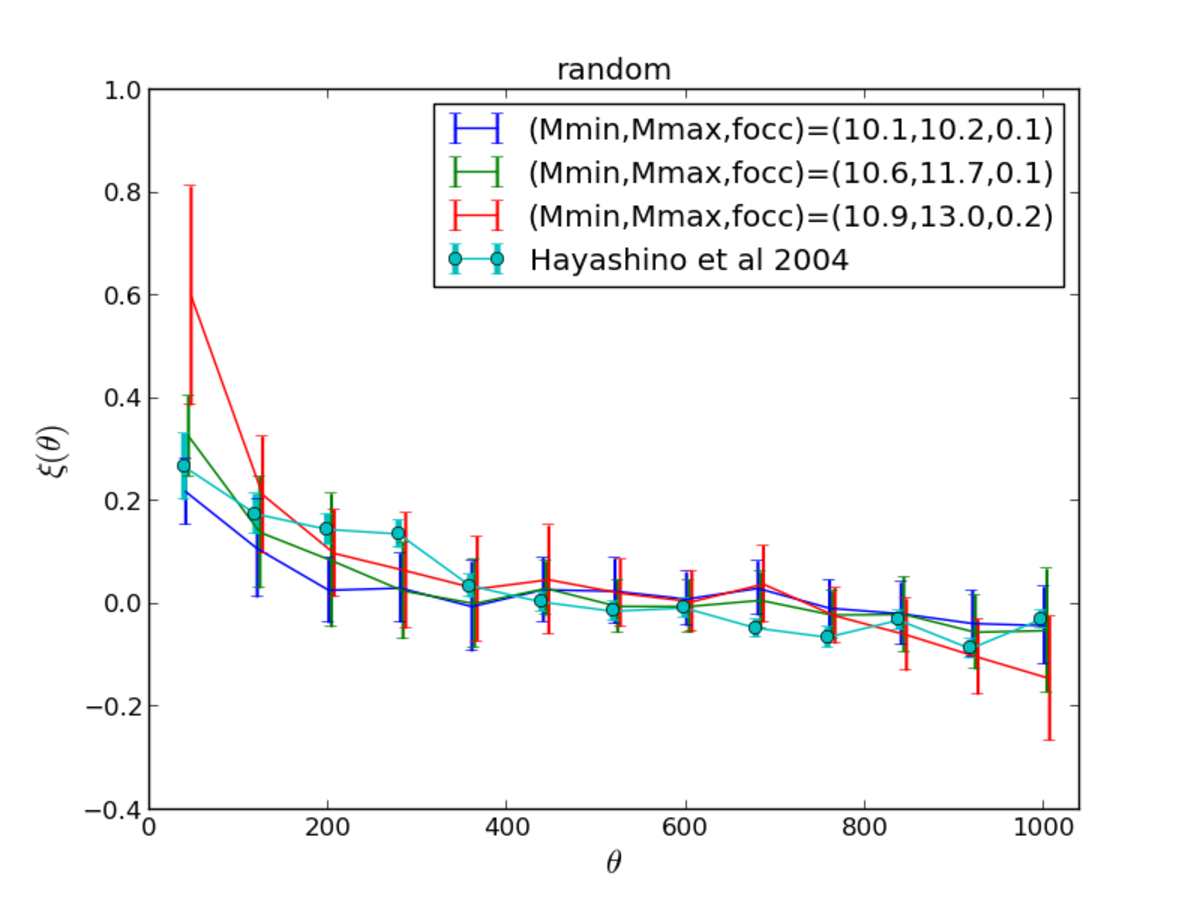
\includegraphics[width=0.46\linewidth,angle=0]{./plots/random_full_correlation_selected_models.pdf}
%\end{center} 
%\caption{ mean ACFs   and their correponding standard deviation (error
%  bars)  of some selected models in different mass ranges over the 7
%  subfields of the SSA22 field (left) and the entire 12 field sample
%  (rigth) using the  random
%  configuration. \label{figure:correlation_random} }   
%\end{figure*}

\section{Discussion}



%\begin{figure*}
%\begin{center}
%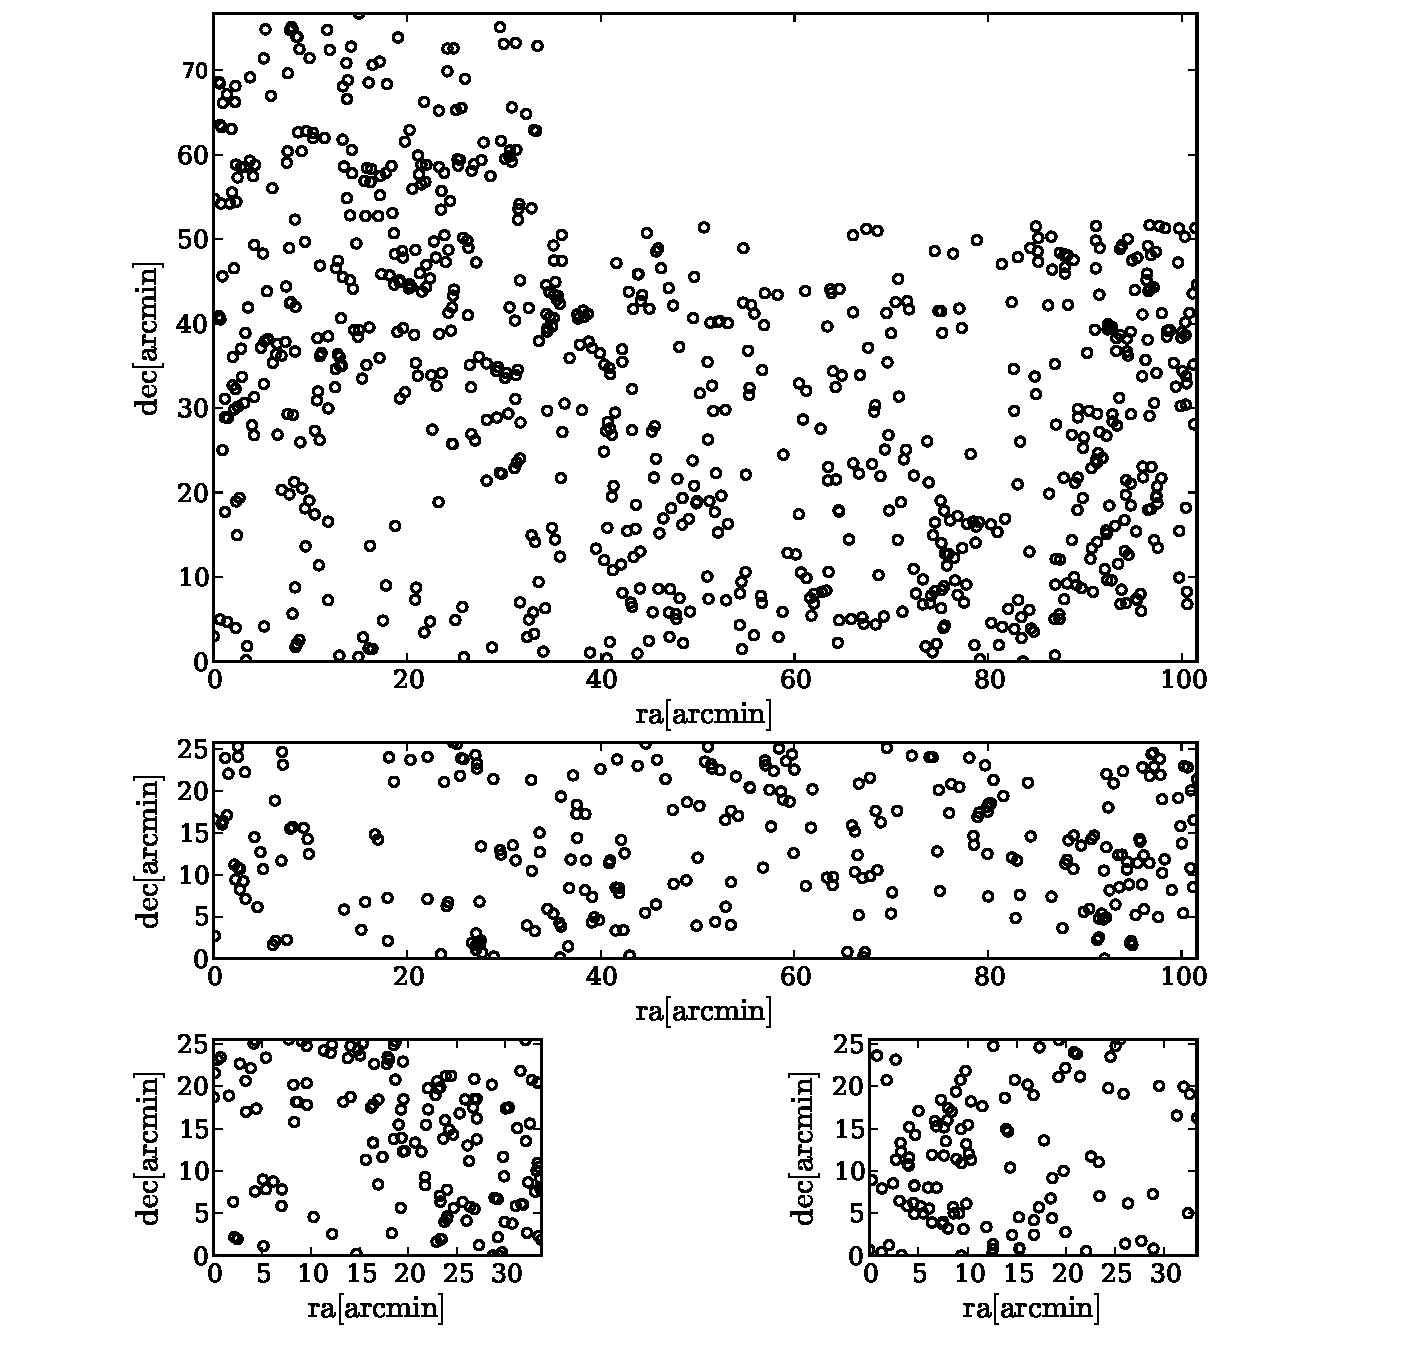
\includegraphics[width=0.49\linewidth,angle=0]{./plots/mytest.pdf}
%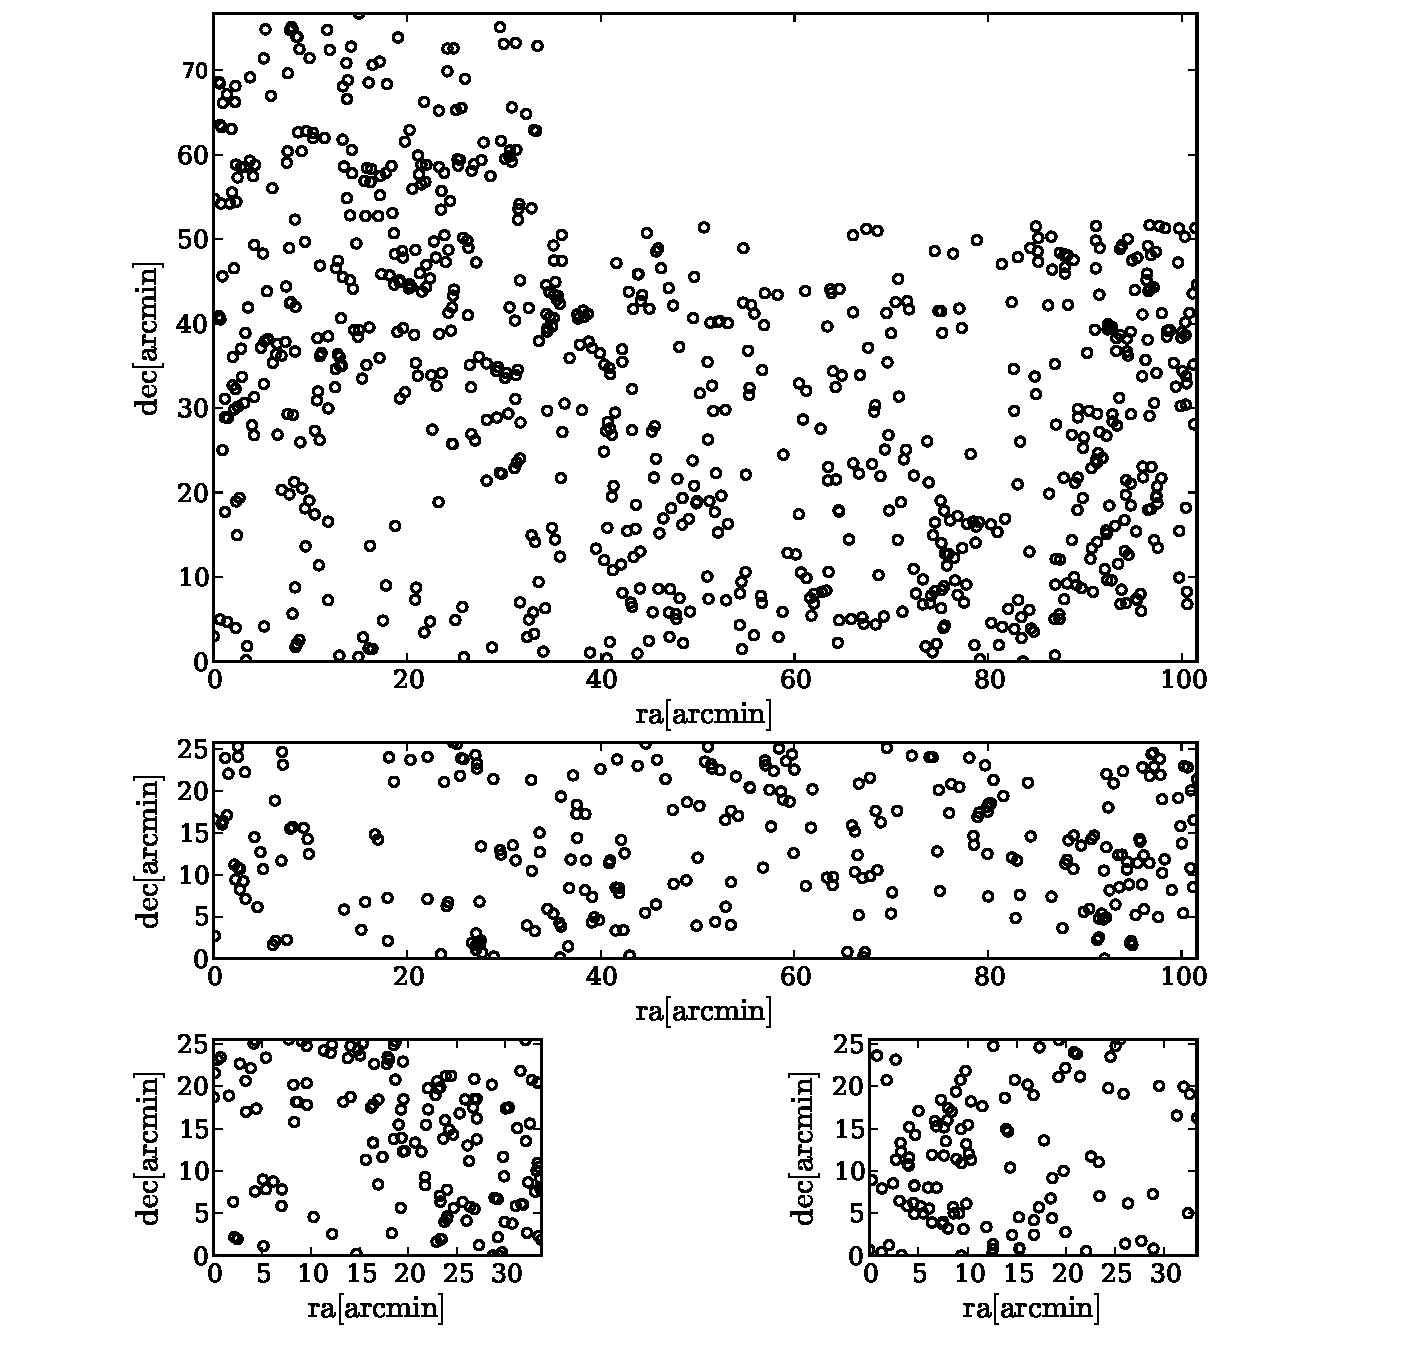
\includegraphics[width=0.49\linewidth,angle=0]{./plots/mytest.pdf}
%\end{center} 
%\caption{Spatial distribution for two mocks corresponding to the model
%  $M_{\rm min}=$, $M_{\rm max}=$ and $f_{\rm occ}=$. All the 15
%  different mock  surveys for this model in the {\texttt match}
%  configuration are consistent with observations at the $P>0.05$
%  level. The full data for all the mocks can be found in the github
%  repository for this paper.
%  \label{figure:spatial_distro}.}
%\end{figure*}


When we include the tightest constraints on the mock catalogs, we find
that there are 30 set of parameters of our model, out of the original
90000 initial models, that are consistent with the observational
constraints at redshift $3.1$: the distribution of the number density,
the inferred values for the average occupation fraction. The
consistency with the angular correlation, in terms of the $\chi^2$
statistics did not help to discard any additional models with a
significant degree of confidence. 


These 30 models can be classified into two families of the same
size. The first, where the range $M_{\rm min}-M_{\rm max}$ is narrow,
typically of less than $<1.0$ dex. While in the second familiy the
extent $>1.0$ dex. In the first case the minimum halo mass is found to
be in a wide range $10^{10}\hMsun <M_{\rm min}< 10^{11.5}\hMsun$ while
in the second case, only models with $M_{\rm min}\sim 10^{10.9}\hMsun$
are compatible with the observational contraints. In what follows we
discuss the implications of the existence of these two families of
models.  

\subsection{Implications for galaxy formation models}

In the case of a narrow of masses to host LAEs the upper masses are
bound to be $M_{\rm max}< 10^{11.5}$\hMsun as it is show in Figure
\ref{figure:mock_and_f_occ}. For halos more massive than this bound it
is naturally expected that the galaxies can be observed as Lyman Break
Galaxies (LBGs). This would imply that not all the bright LBGs can
detected as a LAE.

We have the opposite situation in the second familiy of models. If
we have a wide range in halo masses, where the upper end of the halo
masses can be considered as observed LAEs, one can expect that bright
LBGs will have a correspondence as observed LAEs. The most interesting
aspect is that there is a clear cut in the minimal mass that can be
attained by observed LAEs $M_{\rm min}> 10^{11}$\hMsun. This puts a tight
constraint on the relationship between the minimum star formation rate
required to be observed as a LAE and this minimal halo mass.


... Intrinsic emission and escape fraction.

... Star formation rate efficiency at this redshift.

... Mass dependence of the escape fraction.

... Discuss all this in terms of the star formation efficiency in
Behroozi et al.

\subsection{Implications for large LAEs surveys}

... The bias for the preferred halo mass.

... The scale at which cosmic variance drops.

... This can be observationally tested with HETDEX.

\subsection{On the reproducibility of our results}

... All the software to produce the results in this paper is publicly
available. 

... The raw catalogs can be obtained from the MultiDark database but
can also be obtained in the repository of this paper on github.

\section{Conclusions}
In this \documentname we constrain the preferred mass for dark matter
halos hosting Lyman Alpha Emitters at a redshift $z=3.1$. We use a
method that matches the cosmic variance in the surface
density number of LAEs between mock and real observations. The mock
catalogs are based on a simplified model with three basic parameters: the halo
mass range where LAEs can be found, $M_{\rm   min}<M_{\rm h}<M_{\rm
  max}$, and the fraction of the halos in thisrange that are actully
occupied, $f_{\rm occ}$. After a thorugh exploration of the parameter
space we are able to constrain the mass range of dark matter halos
hosting LAEs to be in the range $<M_{\rm   h}<$ and a corresponding
occupation fraction that escales as $f_{\rm   occ} = M_{\rm min}$. 

We use three additional constraints to reduce the allowed
range of models. The first imposes a tighter criterion to consider a
model succesful, namely that all the mock surveys for a given model
must be consistent with observations. This restriction narrows down
the allowed range of models to be. 

The second constraint is based on the observational results that high
redshift LAEs have a bulk Lyman alpha escape fraction of $XX$ which
can be also interepreted as an average occupation fraction of $XX$.

Including additional observational constraints on the occupation
fraction allows us to reduce the range of allowed halo masses to be in
a narrower range of $<M_{\rm h}<$. Including the information from the
angular correlation function (ACF) does not allows us to impose
further constraints. This is due to the scatter in the ACF due to the
cosmic variance on the field observed by XXX


We simulation allows us to extract $210$ sub-boxes each of which has a
comparable volume to the individual fields of view observed by
\cite{Yamada2012}. The comparison of the observed number density
distribution against the results from our model is based on three
different ways of constructing mock surveys. The first reproduces the
spatial correlation between the $12$ observational fields ({\texttt
  match}), the second breaks this spatial correlation while keeping
the number of fields ({\texttt random}) and the third one simply
includes all the $210$ sub-boxes ({\texttt full}). We find that the
methods {\texttt match} and {\texttt random} allow a larger set of
models than the {{\texttt random}} method. We do not find a
significant difference between the two first methods. 


\section*{Acknowledgments} 


\begin{table}
\begin{center}
\begin{tabular}{ccc}\hline\hline
$\log_{10}M_{\rm min}$ & $\log_{10}M_{\rm max}$ & $f_{\rm occ}$\\\hline
10.1& 10.2& 0.1\\
10.3& 10.5& 0.1\\
10.4& 10.7& 0.1\\
10.5& 10.9& 0.1\\
10.5& 11.0& 0.1\\
10.6& 11.2& 0.1\\
10.6& 11.3& 0.1\\
10.6& 11.4& 0.1\\
10.6& 11.5& 0.1\\
10.6& 11.6& 0.1\\
10.6& 11.7& 0.1\\
10.6& 10.8& 0.2\\
10.7& 11.0& 0.2\\
10.8& 11.2& 0.2\\
10.8& 11.3& 0.2\\
10.8& 11.4& 0.2\\
10.9& 11.7& 0.2\\
10.9& 11.8& 0.2\\
10.9& 11.9& 0.2\\
10.9& 12.0& 0.2\\
10.9& 12.1& 0.2\\
10.9& 12.2& 0.2\\
10.9& 12.3& 0.2\\
10.9& 12.4& 0.2\\
10.9& 12.5& 0.2\\
10.9& 12.6& 0.2\\
10.9& 12.7& 0.2\\
10.9& 12.8& 0.2\\
10.9& 12.9& 0.2\\
10.9& 13.0& 0.2\\\hline\hline
\end{tabular}
\end{center}
\caption{List of model parameters for the best models that have all
  mock surveys consistent with observations and an occupation
  fraction $f_{\rm occ}\leq 0.2$. This corresponds to the {\texttt
    match} method to construct the mock surveys. \label{table:models_match}. }
\end{table}

\bibliographystyle{mn2e}
\bibliography{references} 

\end{document}

lun abr 29 07:38:58 COT 2013
